% Options for packages loaded elsewhere
\PassOptionsToPackage{unicode}{hyperref}
\PassOptionsToPackage{hyphens}{url}
\PassOptionsToPackage{dvipsnames,svgnames,x11names}{xcolor}
%
\documentclass[
  letterpaper,
  DIV=11,
  numbers=noendperiod]{scrartcl}

\usepackage{amsmath,amssymb}
\usepackage{iftex}
\ifPDFTeX
  \usepackage[T1]{fontenc}
  \usepackage[utf8]{inputenc}
  \usepackage{textcomp} % provide euro and other symbols
\else % if luatex or xetex
  \usepackage{unicode-math}
  \defaultfontfeatures{Scale=MatchLowercase}
  \defaultfontfeatures[\rmfamily]{Ligatures=TeX,Scale=1}
\fi
\usepackage{lmodern}
\ifPDFTeX\else  
    % xetex/luatex font selection
\fi
% Use upquote if available, for straight quotes in verbatim environments
\IfFileExists{upquote.sty}{\usepackage{upquote}}{}
\IfFileExists{microtype.sty}{% use microtype if available
  \usepackage[]{microtype}
  \UseMicrotypeSet[protrusion]{basicmath} % disable protrusion for tt fonts
}{}
\makeatletter
\@ifundefined{KOMAClassName}{% if non-KOMA class
  \IfFileExists{parskip.sty}{%
    \usepackage{parskip}
  }{% else
    \setlength{\parindent}{0pt}
    \setlength{\parskip}{6pt plus 2pt minus 1pt}}
}{% if KOMA class
  \KOMAoptions{parskip=half}}
\makeatother
\usepackage{xcolor}
\setlength{\emergencystretch}{3em} % prevent overfull lines
\setcounter{secnumdepth}{-\maxdimen} % remove section numbering
% Make \paragraph and \subparagraph free-standing
\makeatletter
\ifx\paragraph\undefined\else
  \let\oldparagraph\paragraph
  \renewcommand{\paragraph}{
    \@ifstar
      \xxxParagraphStar
      \xxxParagraphNoStar
  }
  \newcommand{\xxxParagraphStar}[1]{\oldparagraph*{#1}\mbox{}}
  \newcommand{\xxxParagraphNoStar}[1]{\oldparagraph{#1}\mbox{}}
\fi
\ifx\subparagraph\undefined\else
  \let\oldsubparagraph\subparagraph
  \renewcommand{\subparagraph}{
    \@ifstar
      \xxxSubParagraphStar
      \xxxSubParagraphNoStar
  }
  \newcommand{\xxxSubParagraphStar}[1]{\oldsubparagraph*{#1}\mbox{}}
  \newcommand{\xxxSubParagraphNoStar}[1]{\oldsubparagraph{#1}\mbox{}}
\fi
\makeatother

\usepackage{color}
\usepackage{fancyvrb}
\newcommand{\VerbBar}{|}
\newcommand{\VERB}{\Verb[commandchars=\\\{\}]}
\DefineVerbatimEnvironment{Highlighting}{Verbatim}{commandchars=\\\{\}}
% Add ',fontsize=\small' for more characters per line
\usepackage{framed}
\definecolor{shadecolor}{RGB}{241,243,245}
\newenvironment{Shaded}{\begin{snugshade}}{\end{snugshade}}
\newcommand{\AlertTok}[1]{\textcolor[rgb]{0.68,0.00,0.00}{#1}}
\newcommand{\AnnotationTok}[1]{\textcolor[rgb]{0.37,0.37,0.37}{#1}}
\newcommand{\AttributeTok}[1]{\textcolor[rgb]{0.40,0.45,0.13}{#1}}
\newcommand{\BaseNTok}[1]{\textcolor[rgb]{0.68,0.00,0.00}{#1}}
\newcommand{\BuiltInTok}[1]{\textcolor[rgb]{0.00,0.23,0.31}{#1}}
\newcommand{\CharTok}[1]{\textcolor[rgb]{0.13,0.47,0.30}{#1}}
\newcommand{\CommentTok}[1]{\textcolor[rgb]{0.37,0.37,0.37}{#1}}
\newcommand{\CommentVarTok}[1]{\textcolor[rgb]{0.37,0.37,0.37}{\textit{#1}}}
\newcommand{\ConstantTok}[1]{\textcolor[rgb]{0.56,0.35,0.01}{#1}}
\newcommand{\ControlFlowTok}[1]{\textcolor[rgb]{0.00,0.23,0.31}{\textbf{#1}}}
\newcommand{\DataTypeTok}[1]{\textcolor[rgb]{0.68,0.00,0.00}{#1}}
\newcommand{\DecValTok}[1]{\textcolor[rgb]{0.68,0.00,0.00}{#1}}
\newcommand{\DocumentationTok}[1]{\textcolor[rgb]{0.37,0.37,0.37}{\textit{#1}}}
\newcommand{\ErrorTok}[1]{\textcolor[rgb]{0.68,0.00,0.00}{#1}}
\newcommand{\ExtensionTok}[1]{\textcolor[rgb]{0.00,0.23,0.31}{#1}}
\newcommand{\FloatTok}[1]{\textcolor[rgb]{0.68,0.00,0.00}{#1}}
\newcommand{\FunctionTok}[1]{\textcolor[rgb]{0.28,0.35,0.67}{#1}}
\newcommand{\ImportTok}[1]{\textcolor[rgb]{0.00,0.46,0.62}{#1}}
\newcommand{\InformationTok}[1]{\textcolor[rgb]{0.37,0.37,0.37}{#1}}
\newcommand{\KeywordTok}[1]{\textcolor[rgb]{0.00,0.23,0.31}{\textbf{#1}}}
\newcommand{\NormalTok}[1]{\textcolor[rgb]{0.00,0.23,0.31}{#1}}
\newcommand{\OperatorTok}[1]{\textcolor[rgb]{0.37,0.37,0.37}{#1}}
\newcommand{\OtherTok}[1]{\textcolor[rgb]{0.00,0.23,0.31}{#1}}
\newcommand{\PreprocessorTok}[1]{\textcolor[rgb]{0.68,0.00,0.00}{#1}}
\newcommand{\RegionMarkerTok}[1]{\textcolor[rgb]{0.00,0.23,0.31}{#1}}
\newcommand{\SpecialCharTok}[1]{\textcolor[rgb]{0.37,0.37,0.37}{#1}}
\newcommand{\SpecialStringTok}[1]{\textcolor[rgb]{0.13,0.47,0.30}{#1}}
\newcommand{\StringTok}[1]{\textcolor[rgb]{0.13,0.47,0.30}{#1}}
\newcommand{\VariableTok}[1]{\textcolor[rgb]{0.07,0.07,0.07}{#1}}
\newcommand{\VerbatimStringTok}[1]{\textcolor[rgb]{0.13,0.47,0.30}{#1}}
\newcommand{\WarningTok}[1]{\textcolor[rgb]{0.37,0.37,0.37}{\textit{#1}}}

\providecommand{\tightlist}{%
  \setlength{\itemsep}{0pt}\setlength{\parskip}{0pt}}\usepackage{longtable,booktabs,array}
\usepackage{calc} % for calculating minipage widths
% Correct order of tables after \paragraph or \subparagraph
\usepackage{etoolbox}
\makeatletter
\patchcmd\longtable{\par}{\if@noskipsec\mbox{}\fi\par}{}{}
\makeatother
% Allow footnotes in longtable head/foot
\IfFileExists{footnotehyper.sty}{\usepackage{footnotehyper}}{\usepackage{footnote}}
\makesavenoteenv{longtable}
\usepackage{graphicx}
\makeatletter
\def\maxwidth{\ifdim\Gin@nat@width>\linewidth\linewidth\else\Gin@nat@width\fi}
\def\maxheight{\ifdim\Gin@nat@height>\textheight\textheight\else\Gin@nat@height\fi}
\makeatother
% Scale images if necessary, so that they will not overflow the page
% margins by default, and it is still possible to overwrite the defaults
% using explicit options in \includegraphics[width, height, ...]{}
\setkeys{Gin}{width=\maxwidth,height=\maxheight,keepaspectratio}
% Set default figure placement to htbp
\makeatletter
\def\fps@figure{htbp}
\makeatother

\usepackage{booktabs}
\usepackage{caption}
\usepackage{longtable}
\usepackage{colortbl}
\usepackage{array}
\KOMAoption{captions}{tableheading}
\makeatletter
\@ifpackageloaded{tcolorbox}{}{\usepackage[skins,breakable]{tcolorbox}}
\@ifpackageloaded{fontawesome5}{}{\usepackage{fontawesome5}}
\definecolor{quarto-callout-color}{HTML}{909090}
\definecolor{quarto-callout-note-color}{HTML}{0758E5}
\definecolor{quarto-callout-important-color}{HTML}{CC1914}
\definecolor{quarto-callout-warning-color}{HTML}{EB9113}
\definecolor{quarto-callout-tip-color}{HTML}{00A047}
\definecolor{quarto-callout-caution-color}{HTML}{FC5300}
\definecolor{quarto-callout-color-frame}{HTML}{acacac}
\definecolor{quarto-callout-note-color-frame}{HTML}{4582ec}
\definecolor{quarto-callout-important-color-frame}{HTML}{d9534f}
\definecolor{quarto-callout-warning-color-frame}{HTML}{f0ad4e}
\definecolor{quarto-callout-tip-color-frame}{HTML}{02b875}
\definecolor{quarto-callout-caution-color-frame}{HTML}{fd7e14}
\makeatother
\makeatletter
\@ifpackageloaded{caption}{}{\usepackage{caption}}
\AtBeginDocument{%
\ifdefined\contentsname
  \renewcommand*\contentsname{Table of contents}
\else
  \newcommand\contentsname{Table of contents}
\fi
\ifdefined\listfigurename
  \renewcommand*\listfigurename{List of Figures}
\else
  \newcommand\listfigurename{List of Figures}
\fi
\ifdefined\listtablename
  \renewcommand*\listtablename{List of Tables}
\else
  \newcommand\listtablename{List of Tables}
\fi
\ifdefined\figurename
  \renewcommand*\figurename{Figure}
\else
  \newcommand\figurename{Figure}
\fi
\ifdefined\tablename
  \renewcommand*\tablename{Table}
\else
  \newcommand\tablename{Table}
\fi
}
\@ifpackageloaded{float}{}{\usepackage{float}}
\floatstyle{ruled}
\@ifundefined{c@chapter}{\newfloat{codelisting}{h}{lop}}{\newfloat{codelisting}{h}{lop}[chapter]}
\floatname{codelisting}{Listing}
\newcommand*\listoflistings{\listof{codelisting}{List of Listings}}
\usepackage{amsthm}
\theoremstyle{definition}
\newtheorem{example}{Example}[section]
\theoremstyle{definition}
\newtheorem{exercise}{Exercise}[section]
\theoremstyle{definition}
\newtheorem{definition}{Definition}[section]
\theoremstyle{remark}
\AtBeginDocument{\renewcommand*{\proofname}{Proof}}
\newtheorem*{remark}{Remark}
\newtheorem*{solution}{Solution}
\newtheorem{refremark}{Remark}[section]
\newtheorem{refsolution}{Solution}[section]
\makeatother
\makeatletter
\makeatother
\makeatletter
\@ifpackageloaded{caption}{}{\usepackage{caption}}
\@ifpackageloaded{subcaption}{}{\usepackage{subcaption}}
\makeatother

\ifLuaTeX
  \usepackage{selnolig}  % disable illegal ligatures
\fi
\usepackage{bookmark}

\IfFileExists{xurl.sty}{\usepackage{xurl}}{} % add URL line breaks if available
\urlstyle{same} % disable monospaced font for URLs
\hypersetup{
  colorlinks=true,
  linkcolor={blue},
  filecolor={Maroon},
  citecolor={Blue},
  urlcolor={Blue},
  pdfcreator={LaTeX via pandoc}}


\author{}
\date{}

\begin{document}


\section{Punktmodelle 1}\label{sec-punktmodelle1}

\subsection{Lernsteuerung}\label{lernsteuerung}

\subsubsection{Standort im Lernpfad}\label{standort-im-lernpfad}

\textbf{?@fig-ueberblick} zeigt den Standort dieses Kapitels im Lernpfad
und gibt damit einen Überblick über das Thema dieses Kapitels im Kontext
aller Kapitel.

\subsubsection{Lernziele}\label{lernziele}

\begin{itemize}
\tightlist
\item
  Sie können gängige Arten von Lagemaße definieren.
\item
  Sie können erläutern, inwiefern man ein Lagemaß als ein Modell
  hernehmen kann.
\item
  Sie können Lagemaße mit R berechnen.
\end{itemize}

\subsubsection{Benötigte R-Pakete}\label{benuxf6tigte-r-pakete}

In diesem Kapitel benötigen Sie folgende R-Pakete.

\begin{Shaded}
\begin{Highlighting}[]
\FunctionTok{library}\NormalTok{(tidyverse)}
\end{Highlighting}
\end{Shaded}

\begin{verbatim}
-- Attaching core tidyverse packages ---- tidyverse 2.0.0 --
v dplyr     1.1.4     v readr     2.1.5
v forcats   1.0.0     v stringr   1.5.1
v ggplot2   3.5.1     v tibble    3.2.1
v lubridate 1.9.3     v tidyr     1.3.1
v purrr     1.0.2     
-- Conflicts ---------------------- tidyverse_conflicts() --
x dplyr::filter() masks stats::filter()
x dplyr::lag()    masks stats::lag()
i Use the conflicted package (<http://conflicted.r-lib.org/>) to force all conflicts to become errors
\end{verbatim}

\begin{Shaded}
\begin{Highlighting}[]
\FunctionTok{library}\NormalTok{(easystats)}
\end{Highlighting}
\end{Shaded}

\begin{verbatim}
# Attaching packages: easystats 0.7.1 (red = needs update)
x bayestestR  0.13.2    x correlation 0.8.4  
x datawizard  0.10.0    x effectsize  0.8.7  
x insight     0.19.10   x modelbased  0.8.7  
x performance 0.11.0    x parameters  0.21.6 
x report      0.5.8     x see         0.8.3  

Restart the R-Session and update packages with `easystats::easystats_update()`.
\end{verbatim}

\subsubsection{Benötigte Daten}\label{benuxf6tigte-daten}

\begin{Shaded}
\begin{Highlighting}[]
\NormalTok{mariokart }\OtherTok{\textless{}{-}} \FunctionTok{read.csv}\NormalTok{(}\StringTok{"https://vincentarelbundock.github.io/Rdatasets/csv/openintro/mariokart.csv"}\NormalTok{)}
\end{Highlighting}
\end{Shaded}

\subsection{Mittelwert als Modell}\label{sec-mw}

Der klassische Mittelwert (arithmetisches Mittel) ist ein prototypisches
Beispiel für ein Modell in der Statistik.

\begin{exercise}[]\protect\hypertarget{exr-mw-md-mod}{}\label{exr-mw-md-mod}

Welche Vorstellung haben Sie, wenn Sie hören, dass der ``typische
deutsche Mann'' 1,80m groß ist {[}@owidhumanheight{]}?\footnote{Ihr
  Vorstellung updatet sich in Definition~\ref{def-mw}.}

\begin{enumerate}
\def\labelenumi{\alph{enumi})}
\tightlist
\item
  Die Hälfte der Männer ist größer als 1,80m, die andere Hälfte kleiner.
\item
  Das arithmetische Mittel der Männer beträgt 1,80m.
\item
  Die meisten Männer sind 1,80m groß.
\item
  Etwas anderes.
\item
  Keine Ahnung! \(\square\)
\end{enumerate}

\end{exercise}

\begin{exercise}[]\protect\hypertarget{exr-mw2}{}\label{exr-mw2}

Laut
\href{https://en.wikipedia.org/wiki/Average_human_height_by_country}{dieser
Quelle} beträgt der Wert der mittleren Größe deutscher Frauen etwa
1,66m, also 14 cm weniger als bei Männern.\footnote{\url{https://en.wikipedia.org/wiki/Average_human_height_by_country}}
\(\square\)

\end{exercise}

\subsubsection{Frage}

Ist das viel?

\begin{enumerate}
\def\labelenumi{\alph{enumi})}
\tightlist
\item
  ja
\item
  nein
\item
  kommt drauf an
\item
  weiß nicht \(\square\)
\end{enumerate}

\subsubsection{Antwort}

Auf dieser Frage gibt es keine Antwort, zumindest nicht ohne weitere
Annahmen. So könnte man z.B. sagen, ``mehr als 5 cm sind viel''. So eine
Entscheidung ist aber keine statistische Angelegenheit, sondern eine
inhaltliche.

\begin{example}[Beispiel zum
Mittelwert]\protect\hypertarget{exm-mw}{}\label{exm-mw}

Ein Statistikkurs besteht aus drei Studentinnen: Anna, Berta und Carla.
Sie haben gerade ihre Noten in der Klausur erfahren. Anna hat eine 1,
Berta eine 2 und Carla eine 3. Der Durchschnitt (das arithmetische
Mittel, \(\varnothing\)) beträgt: 2. \(\square\)

\end{example}

\begin{quote}
🧑‍🎓 Zu easy!
\end{quote}

\begin{quote}
👨‍🏫 Schon gut! Chill mal. Wird gleich interessanter.
\end{quote}

Die Rechenregel zum Mittelwert lautet:

\begin{enumerate}
\def\labelenumi{\arabic{enumi}.}
\tightlist
\item
  Addiere alle Werte
\item
  Teile durch die Anzahl der Werte
\item
  Fertig. 😄
\end{enumerate}

Etwas abstrakter kann man Example~\ref{exm-mw} in folgendem Schaubild
darstellen, s. Equation~\ref{eq-mw}.

\begin{equation}\phantomsection\label{eq-mw}{
\begin{array}{|c|} \hline \\ \\ \square \\ \hline \end{array} + \begin{array}{|c|} \hline \\ \square \\ \square \\ \hline \end{array} + \begin{array}{|c|} \hline \square \\ \square \\ \square \\ \hline \end{array} = 3 \cdot \begin{array}{|c|} \hline \\ \square \\ \square \\ \hline \end{array}
}\end{equation}

Der Nutzen des Mittelwerts liegt darin, dass er uns ein Bild gibt (ein
Modell ist!) für die ``typische Note'' im Statistikkurs, s.
Equation~\ref{eq-mw2}.

\begin{equation}\phantomsection\label{eq-mw2}{\begin{array}{|c|} \hline \\ \\ \square \\ \hline \end{array} + \begin{array}{|c|} \hline \\ \square \\ \square \\ \hline \end{array} + \begin{array}{|c|} \hline \square \\ \square \\ \square \\ \hline \end{array} \qquad \leftrightarrow  \qquad \underbrace{\begin{array}{|c|} \hline \\ \square \\ \square \\ \hline \end{array}}_{\text{"typischer Vertreter"}}}\end{equation}

\begin{tcolorbox}[enhanced jigsaw, breakable, toptitle=1mm, colback=white, leftrule=.75mm, colframe=quarto-callout-important-color-frame, colbacktitle=quarto-callout-important-color!10!white, title=\textcolor{quarto-callout-important-color}{\faExclamation}\hspace{0.5em}{Important}, toprule=.15mm, opacityback=0, arc=.35mm, coltitle=black, rightrule=.15mm, titlerule=0mm, bottomtitle=1mm, bottomrule=.15mm, left=2mm, opacitybacktitle=0.6]

Der Nutzen des Mittelwerts liegt darin, dass er eine Datenreihe zu einen
``typischen Vertreter'' zusammenfasst. Er ist typisch in dem Sinne, als
dass die Werte aller Merkmalsträger in gleichem Maße einfließen. Er gibt
uns eine (mögliche) Vorstellung (ein Modell!), wie wir uns die Werte der
Datenreihe vorstellen sollen.

\end{tcolorbox}

Eine nützliche Anschauung zum Mittelwert ist die Vorstellung des
Mittelwerts als eine ausbalancierte Wippe, s. Figure~\ref{fig-wippe}.

\begin{figure}

\centering{

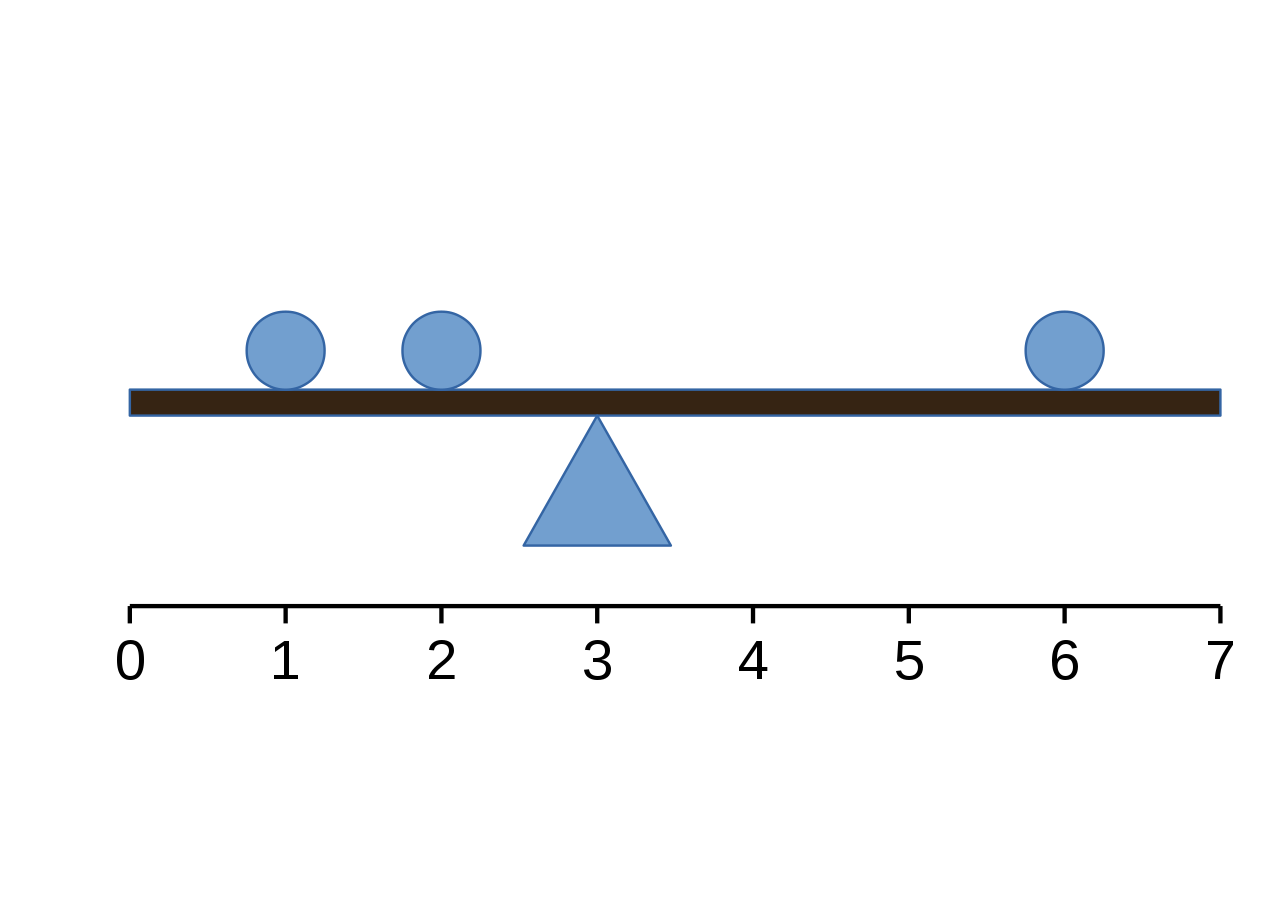
\includegraphics[width=0.7\textwidth,height=\textheight]{img/1280px-Seesaw_with_mean.svg.png}

}

\caption{\label{fig-wippe}Mittelwert als ausbalancierte Wippe mit
Mittelwert 3}

\end{figure}%

\href{https://commons.wikimedia.org/w/index.php?curid=79390659}{Quelle:
Von Maphry - Eigenes Werk, CC BY-SA 4.0}

In ``Mathe-Sprech'' bezeichnet man den Mittelwert häufig mit \(\bar{x}\)
und schreibt die Rechenregel so, s. Equation~\ref{eq-mw-formel}.

\begin{equation}\phantomsection\label{eq-mw-formel}{\bar {x} =\frac{1}{n} \sum_{i=1}^{n}{x_{i}}=\frac {x_{1}+x_{2}+\dotsb +x_{n}} {n}}\end{equation}

\begin{definition}[Mittelwert]\protect\hypertarget{def-mw}{}\label{def-mw}

Der Mittelwert der Variablen \(X\) (präziser: das arithmetische Mittel
von \(X\)) ist definiert als die Summe der Elemente von \(X\) geteilt
durch deren Anzahl, \(n\). Den Mittelwert von \(X\) bezeichnet man mit
\(\bar {x}\). \(\square\)

\end{definition}

Da der Mittelwert eine zentrale Rolle spielt in der Statistik, sollten
wir ihn uns noch etwas genauer anschauen. In s. Figure~\ref{fig-mw1}
sehen wir die Noten von (dieses Mal) vier Studentis. Die gestrichelte
horizontale Linie zeigt den Mittelwert der vier Noten. Die schwarzen
Punkte sind die Daten, in dem Fall die einzelnen Noten. Die vertikalen
Linien zeigen die Abweichungen der Noten zum Mittelwert. Bezeichnen wir
die Abweichung - auch als ``Fehler'', ``Rest'' oder ``Residuum''
bezeichnet - der \(i\)-ten Person mit

\(e_i\)

(\emph{e} wie engl. \emph{error}, Fehler) und die \(i\)-te Note mit
\(\color{ycol}{y_i}\), so können wir mit Equation~\ref{eq-modell1}
festhalten:

\begin{equation}\phantomsection\label{eq-modell1}{\color{ycol}{\text{y}_i} \color{black}{ = } \color{modelcol}{\;\bar{x}\;} + \color{errorcol}{\;\text{e}_i}}\end{equation}

Anders ausgedrückt (s. Equation~\ref{eq-modell2}):

\begin{equation}\phantomsection\label{eq-modell2}{\color{ycol}{\text{Daten}} \color{black}{ = }     \color{modelcol}{\text{Modell}} + 
\color{errorcol}{\text{Rest}}}\end{equation}

Der Mittelwert ist hier unser Modell der Daten. Wie gesagt: Ein Modell
ist eine vereinfachte (zusammengefasste) Beschreibung einer Datenreihe.

Um Modelle darzustellen, wird in der Datenanalyse häufig folgende Art
von Modellgleichung verwendet, s. Equation~\ref{eq-sim-mean}.

\begin{equation}\phantomsection\label{eq-sim-mean}{\color{modelcol}{\hat{y}} \sim \color{xcol}{\text{ x}}}\end{equation}

Lies: ``Der Modellwert \(\color{modelcol}{\hat{y}}\) ist eine Funktion
der Variable \(\color{xcol}{\text{x}}\)''. Der Kringel
``\textasciitilde{}''\footnote{Das ``Kringel'' oder die ``Welle''
  ``\textasciitilde{}'' nennt man auch ``Tilde''.} soll also hier heißen
``\ldots{} ist eine Funktion von \ldots{}''.

Mit \(\color{modelcol}{\hat{y}}\) ist die vorhergesagte bzw. die zu
erklärende Variable\footnote{AV, Output-Variable, Zielvariable} gemeint.
Das ``Dach'' über dem \(\color{ycol}{\text{y}}\) bedeutet
``vorhergesagter Y-Wert'' oder ``Y-Wert laut dem Modell''. Der
tatsächliche, beobachtete Wert \(\color{ycol}{\text{y}}\) setzt sich
zusammen aus dem Modellwert \(\color{modelcol}{\text{m}}\) plus einem
Fehler \(\color{errorcol}{\text{e}}\), s. Equation~\ref{eq-modell3}.

\begin{equation}\phantomsection\label{eq-modell3}{\color{ycol}{y} \color{black}{ = } \color{modelcol}{\text{m}} + \color{errorcol}{\text{e}}}\end{equation}

Anstelle von \(\color{modelcol}{\text{m}}\) schreibt man auch
\(\color{modelcol}{\hat{y}}\) (``y-Dach''). In diesem Fall ist das
Modell einfach gleich dem Mittelwert (und nicht irgendeiner Funktion des
Mittelwerts), so dass wir mit Equation~\ref{eq-modell4} schreiben
können:

\begin{equation}\phantomsection\label{eq-modell4}{\color{ycol}{y}  \color{black}{ = } \color{modelcol}{\bar{x}} + \color{errorcol}{e}}\end{equation}

Die Zielvariable \(\color{ycol}{\text{y}}\) wird also durch ihren
eigenen Mittelwert erklärt, außer gehen wir von einem Fehler \(e\) in
unseren Modellvorhersagen aus. Nobody is perfect. In späteren Kapiteln
werden wir andere Variablen heranziehen, um die Zielvariable zu
erklären. Würden wir z.B. sagen wollen, dass wir
\(\color{ycol}{\text{y}}\) als Funktion einer Variable
\(\color{xcol}{X}\) erklären, so würden wir schreiben (s.
Equation~\ref{eq-modell5a}):

\begin{equation}\phantomsection\label{eq-modell5a}{\color{modelcol}{\bar{y}} \color{black}{ \sim } \color{xcol}{\text{x}}}\end{equation}

Da wir im Moment aber keine andere Variablen bemühen, um
\(\color{ycol}{\text{y}}\) zu erklären, schreibt man mit
Equation~\ref{eq-modell5} auch:

\begin{equation}\phantomsection\label{eq-modell5}{\color{modelcol}{\bar{y}}\;  \color{black}{\sim \; 1}}\end{equation}

Diese Schreibweise sieht verwirrend aus. Die \(1\) soll aber nur zeigen,
dass wir keine andere Variable zur Erklärung von
\(\color{ycol}{\text{y}}\) verwenden, daher steht hier kein Buchstabe,
sondern eine einfache \(1\).\footnote{Der mathematische Hintergrund
  liegt in der Art, wie man Matrizen multipliziert.}

\begin{example}[Noten, Mittelwert und
Abweichung]\protect\hypertarget{exm-noten}{}\label{exm-noten}

Vier Studentis -- Anna, Berta, Carl, Dani -- haben ihre
Statistik-Klausur zurückbekommen (Schluck). Die Noten sehen Sie in
Figure~\ref{fig-mw1}, gar nicht so schlecht ausgefallen. Außerdem ist
der Mittelwert (gestrichelte horizontale Linie) sowie die Abweichungen
der einzelnen Noten vom Mittelwert eingezeichnet.\(\square\)

\end{example}

Schauen Sie sich die Abweichungsbalken\footnote{Residuen, Fehler; häufig
  mit \(e\) wie \emph{error} bezeichnet} in Figure~\ref{fig-mw1} einmal
genauer an.

\begin{figure}

\centering{

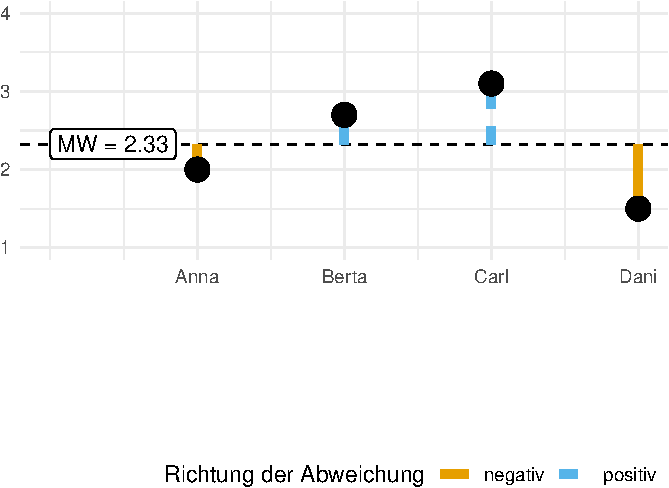
\includegraphics{050-zusammenfassen_files/figure-pdf/fig-mw1-1.pdf}

}

\caption{\label{fig-mw1}Der Mittelwert als horizontale (gestrichelte)
Linie. Die vertikalen Linien zeigen die Abweichungen der einzelnen Werte
zum Mittelwert. Die Abweichungen summieren sich zu Null auf.}

\end{figure}%

Jetzt stellen Sie sich vor, Sie würden die vom Mittelwert nach
\emph{oben} ragenden Balkenlängen aneinanderlegen (das sind die
gestrichelten. Sehen Sie das vor Ihrem geistigen Auge? Jetzt legen Sie
auch noch die Abweichungsbalken, die nach \emph{unten} ragen, aneinander
(die mit den durchgezogenen Linien). Wer viel Phantasie hat, erkennt
(sieht) jetzt, dass die Gesamtlänge der ``Balken nach oben'' identisch
ist zur Gesamtlänge der nach ``unten ragenden Balken'', vgl.
Figure~\ref{fig-wippe}.

Präziser ausgedrückt und ohne Ihre Phantasie zu strapazieren
(Equation~\ref{eq-summenull}):

\begin{equation}\phantomsection\label{eq-summenull}{\sum_{i=1}^n (x_i-\bar{x})=\sum_{i=1}^n x_i - \sum_{i=1}^n \bar{x} = n\cdot \bar{x} - n\cdot \bar{x}=0}\end{equation}

\begin{tcolorbox}[enhanced jigsaw, breakable, toptitle=1mm, colback=white, leftrule=.75mm, colframe=quarto-callout-note-color-frame, colbacktitle=quarto-callout-note-color!10!white, title=\textcolor{quarto-callout-note-color}{\faInfo}\hspace{0.5em}{Note}, toprule=.15mm, opacityback=0, arc=.35mm, coltitle=black, rightrule=.15mm, titlerule=0mm, bottomtitle=1mm, bottomrule=.15mm, left=2mm, opacitybacktitle=0.6]

Die Summe der Abweichungen vom Mittelwert ist Null.

\end{tcolorbox}

\begin{exercise}[]\protect\hypertarget{exr-mw-wealth1}{}\label{exr-mw-wealth1}

Was schätzen Sie, wie hoch das ``mittlere'' Vermögen der Haushalte in
Deutschland in etwa ist?\footnote{Quelle: SI,
  \url{https://www.wsi.de/en/how-is-wealth-distributed-in-germany-14401.html},
  Abruf 2023-04-19}. \(\square\)

\end{exercise}

\subsubsection{Auswahl}

\begin{enumerate}
\def\labelenumi{\alph{enumi})}
\tightlist
\item
  50.000 Euro
\item
  100.000 Euro
\item
  150.000 Euro
\item
  200.000 Euro
\item
  250.000 Euro
\end{enumerate}

\subsubsection{Antwort}

\begin{enumerate}
\def\labelenumi{\alph{enumi})}
\tightlist
\item
  \textbf{50.000 Euro}, ca. 60.000 Euro (laut der o.g. Quelle)
\item
  100.000 Euro
\item
  150.000 Euro
\item
  200.000 Euro
\item
  250.000 Euro
\end{enumerate}

\begin{example}[Der reichste Mensch der Welt in Ihrem
Hörsaal]\protect\hypertarget{exm-md}{}\label{exm-md}

Kommt der wertvollste Fußballspieler der Welt in Ihren Hörsaal, sagen
wir, es ist Kylian Mbappé\footnote{Quelle:
  \url{https://www.transfermarkt.de/spieler-statistik/wertvollstespieler/marktwertetop},
  Abruf 2023-03-19}. Sein Jahreseinkommen (2023) liegt bei ca. 120
Millionen Euro\footnote{Quelle:
  \url{https://www.einkommenmagazin.de/kylian-mbappe-einkommen/}, Abruf
  2023-03-19}.

\begin{quote}
{\emoji{supervillain}} Hey Leute, wie geht's denn so! Wie viel Kohle
verdient ihr eigentlich so?
\end{quote}

\begin{quote}
{\emoji{student}} Äh, wir studieren und verdienen fast nix!
\end{quote}

Die 100 Studis im Hörsaal schauen verdattert aus der Wäsche: Was ist das
für eine komische Frage!? Aber zumindest verteilt der Fußballspieler
Autogramme.

\end{example}

\begin{exercise}[Mittleres Einkommen im Hörsaal, mit Kylian
Mbappé]\protect\hypertarget{exr-elon}{}\label{exr-elon}

Schätzen Sie -- im Kopf -- das mittlere Vermögen im Hörsaal, gehen Sie
davon aus, dass alle der 100 Studentis jeweils 1000 Euro im Jahr
verdienen. \(\square\)

\end{exercise}

In R kann man das mittlere Einkommen (präziser: das arithmetische Mittel
des Einkommens) wie folgt berechnen, s.
Listing~\ref{lst-einkommen}.\footnote{Die Details der Syntax, z.B. der
  Befehl \texttt{rep()}, sind von geringer Bedeutung.}

\begin{codelisting}

\caption{\label{lst-einkommen}Wir simulieren Einkommen von 100 Studis
plus Mbappé.}

\centering{

\begin{Shaded}
\begin{Highlighting}[]
\FunctionTok{set.seed}\NormalTok{(}\DecValTok{42}\NormalTok{)  }\CommentTok{\# Zufallszahlen festlegen, hier nicht so wichtig}
\NormalTok{einkommen\_studis }\OtherTok{\textless{}{-}} \FunctionTok{rep}\NormalTok{(}\AttributeTok{x =} \DecValTok{1000}\NormalTok{, }\AttributeTok{times =} \DecValTok{100}\NormalTok{)  }\CommentTok{\# "rep" wie "repeat": wiederhole 1000 USD 100 Mal}
\NormalTok{einkommen }\OtherTok{\textless{}{-}} \FunctionTok{c}\NormalTok{(einkommen\_studis, }\DecValTok{120}\SpecialCharTok{*}\FloatTok{1e6}\NormalTok{)  }\CommentTok{\# 100 Studis mit 1000, 1 Mbappé mit 120 Mio}
\NormalTok{einkommen\_mw }\OtherTok{\textless{}{-}} \FunctionTok{mean}\NormalTok{(einkommen)}
\NormalTok{einkommen\_mw}
\end{Highlighting}
\end{Shaded}

\begin{verbatim}
[1] 1189109
\end{verbatim}

}

\end{codelisting}%

\begin{tcolorbox}[enhanced jigsaw, breakable, toptitle=1mm, colback=white, leftrule=.75mm, colframe=quarto-callout-note-color-frame, colbacktitle=quarto-callout-note-color!10!white, title=\textcolor{quarto-callout-note-color}{\faInfo}\hspace{0.5em}{Note}, toprule=.15mm, opacityback=0, arc=.35mm, coltitle=black, rightrule=.15mm, titlerule=0mm, bottomtitle=1mm, bottomrule=.15mm, left=2mm, opacitybacktitle=0.6]

1 Million hat 6 Nuller hinter der führenden Eins: 1000000. In
Taschenrechner- oder Computerschreibweise: 1 Mio = \texttt{1e6}, das
\texttt{1e6} ist zu lesen als ``1 Mal 10 hoch 6, also mit 6 im
\emph{E}xponenten''.

\end{tcolorbox}

Der Mittelwert im Hörsaal beträgt also 1,189,109 Euro. Ist das ein gutes
Modell für das ``typische'' Vermögen im Hörsaal?

\subsubsection{Der Mittelwert als lineares
Modell}\label{der-mittelwert-als-lineares-modell}

Man kann den Mittelwert als Gerade einzeichnen, s. Figure~\ref{fig-mw2},
bzw. als Gerade begreifen. Insofern kann man vom Mittelwert auch als
\emph{lineares Modell} sprechen.

\begin{definition}[Lineares
Modell]\protect\hypertarget{def-lm}{}\label{def-lm}

Ein lineares Modell verwendet eine Gerade als Modell der Daten. Es
erklärt die Daten anhand einer Geraden. \(\square\)

\end{definition}

\begin{figure}

\begin{minipage}{0.50\linewidth}

\centering{

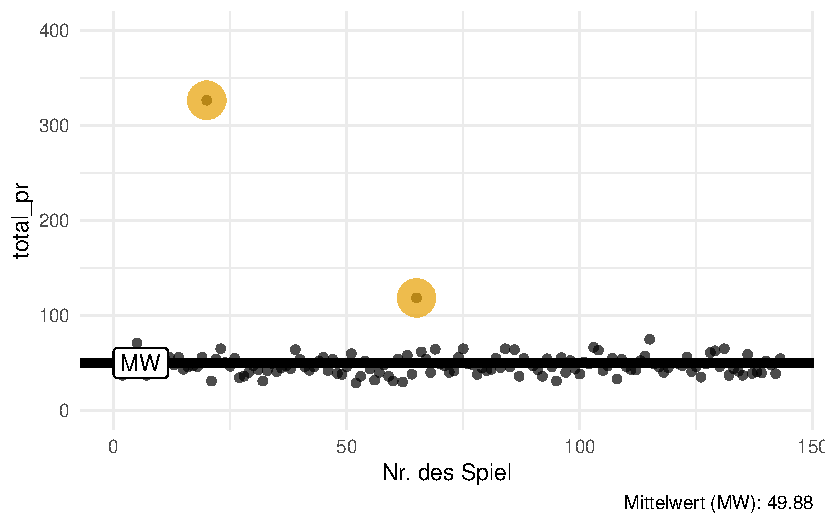
\includegraphics{050-zusammenfassen_files/figure-pdf/fig-mw2-1.pdf}

}

\subcaption{\label{fig-mw2-1}Mit Extremwerten}

\end{minipage}%
%
\begin{minipage}{0.50\linewidth}

\centering{

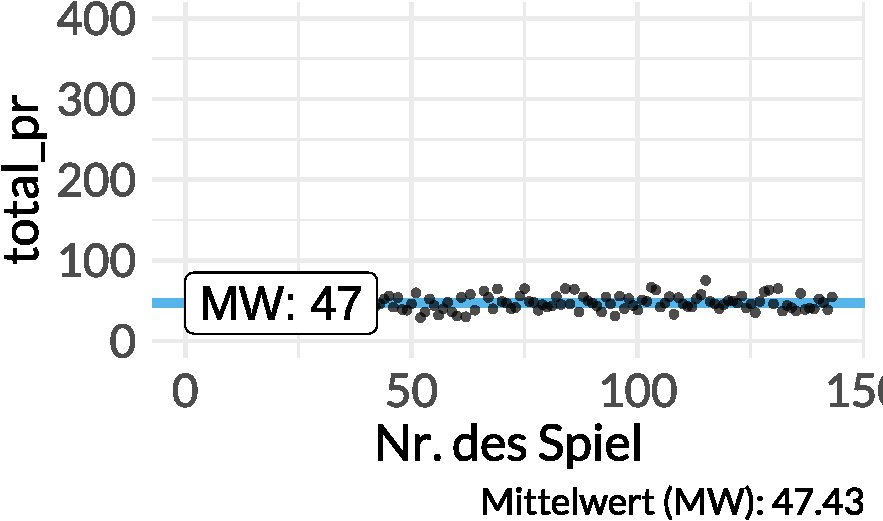
\includegraphics{050-zusammenfassen_files/figure-pdf/fig-mw2-2.pdf}

}

\subcaption{\label{fig-mw2-2}Ohne Extremwerte (\textless100 Euro)}

\end{minipage}%

\caption{\label{fig-mw2}Der mittlere Preis von Mariokart-Spielen als
horizontale Gerade eingezeichnet}

\end{figure}%

Figure~\ref{fig-mw2} zeigt den Mittelwert des Verkaufspreises der
Mariokart-Spiele (\texttt{total\_pr}), einmal mit Extremwerte (a) bzw.
einmal ohne Extremwerte (b).

\begin{definition}[Extremwert]\protect\hypertarget{def-extremwert}{}\label{def-extremwert}

Ein Extremwert (engl. \emph{outlier}) ist eine Beobachtung, dessen Wert
deutlich vom Großteil der anderen Beobachtungen im Datensatz abweicht,
z.B. viel größer ist. \(\square\)

\end{definition}

Berechnen wir mal den Mittelwert von \texttt{einkommen} mit R (vgl.
Listing~\ref{lst-einkommen}):

\begin{Shaded}
\begin{Highlighting}[]
\FunctionTok{lm}\NormalTok{(einkommen }\SpecialCharTok{\textasciitilde{}} \DecValTok{1}\NormalTok{)  }\CommentTok{\# lm wie "lineares Modell" oder engl. "linear modell"}
\end{Highlighting}
\end{Shaded}

\begin{verbatim}

Call:
lm(formula = einkommen ~ 1)

Coefficients:
(Intercept)  
    1189109  
\end{verbatim}

Der Befehl gibt als \emph{Koeffizient} einen Wert zurück und zwar den
Mittelwert von \texttt{einkommen}, Listing~\ref{lst-einkommen}. Dieser
Wert wird als Achsenabschnitt (engl. \emph{intercept}) bezeichnet, das
wird verständlich, wenn man z.B. in Figure~\ref{fig-mw2} sieht, dass die
Gerade (des Mittelwerts) genau an diesem Punkt die Y-Achse schneidet.

Die Syntax des Befehls \texttt{lm()} sieht etwas merkwürdig aus.
Ignorieren Sie das fürs Erste, wir besprechen das später
(\textbf{?@sec-gerade1}) ausführlich. \texttt{lm} steht übrigens für
``lineares Modell''.

\subsection{Median als Modell}\label{sec-median}

\begin{quote}
{\emoji{student}} Hey, der Mittelwert ist doch Quatsch! Das ist gar kein
typischer Wert für die Menschen im Hörsaal. Weder für den Mbappé, noch
für uns Studis!
\end{quote}

\begin{quote}
{\emoji{teacher}} Ja, da habt ihr Recht.
\end{quote}

\begin{quote}
{\emoji{soccer-ball}} Die Welt ist schon ungerecht!
\end{quote}

\begin{tcolorbox}[enhanced jigsaw, breakable, toptitle=1mm, colback=white, leftrule=.75mm, colframe=quarto-callout-important-color-frame, colbacktitle=quarto-callout-important-color!10!white, title=\textcolor{quarto-callout-important-color}{\faExclamation}\hspace{0.5em}{Important}, toprule=.15mm, opacityback=0, arc=.35mm, coltitle=black, rightrule=.15mm, titlerule=0mm, bottomtitle=1mm, bottomrule=.15mm, left=2mm, opacitybacktitle=0.6]

Bei (sehr) schiefen Verteilungen (s. Figure~\ref{fig-mbappe}) ist der
Mittelwert (sehr) wenig aussagekräftig, da er nicht mehr ``typische''
Werte für die Merkmalsträger beschreibt.

\end{tcolorbox}

Figure~\ref{fig-mbappe} stellt die Verteilung einer mit ``normal''
skalierter Achse und einmal mit logarithmischer X-Achse. Die
logarithmische X-Achse stellt den Unterschied von Mittelwert (MW) und
Median deutlicher heraus als die normale (additive) Achse.

\begin{verbatim}
`stat_bin()` using `bins = 30`. Pick better value with
`binwidth`.
`stat_bin()` using `bins = 30`. Pick better value with
`binwidth`.
\end{verbatim}

\begin{figure}

\begin{minipage}{\linewidth}

\centering{

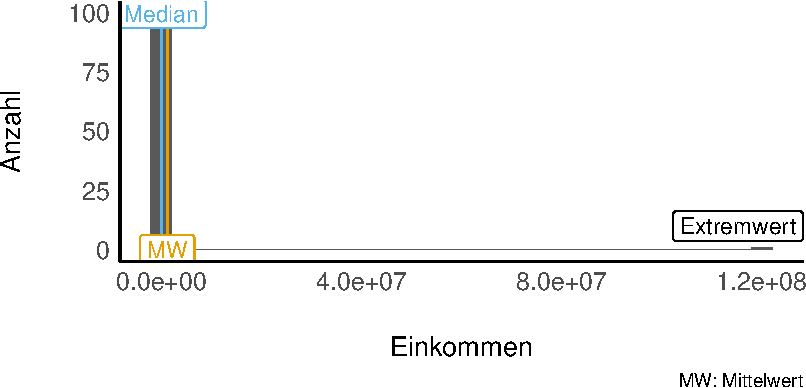
\includegraphics{050-zusammenfassen_files/figure-pdf/fig-mbappe-1.pdf}

}

\subcaption{\label{fig-mbappe-1}X-Achse in additiver Form}

\end{minipage}%
\newline
\begin{minipage}{\linewidth}

\centering{

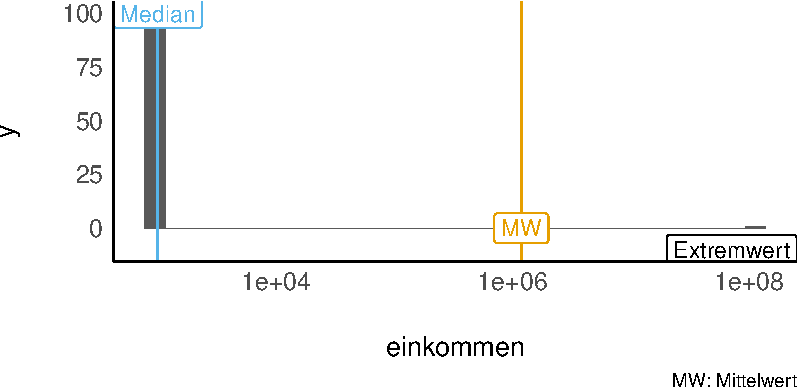
\includegraphics{050-zusammenfassen_files/figure-pdf/fig-mbappe-2.pdf}

}

\subcaption{\label{fig-mbappe-2}X-Achse in multiplikativer Form
(logarithmische Darstellung)}

\end{minipage}%

\caption{\label{fig-mbappe}Die Einkommensverteilung im Hörsaal}

\end{figure}%

Der Mittelwert ist Hörsaal ist nicht typisch für die Menschen im
Hörsaal: Weder für Mbappé, noch für die Studis. Genau genommen ist der
Mittelwert in diesem Fall ziemlich nutzlos.

\begin{tcolorbox}[enhanced jigsaw, breakable, toptitle=1mm, colback=white, leftrule=.75mm, colframe=quarto-callout-important-color-frame, colbacktitle=quarto-callout-important-color!10!white, title=\textcolor{quarto-callout-important-color}{\faExclamation}\hspace{0.5em}{Important}, toprule=.15mm, opacityback=0, arc=.35mm, coltitle=black, rightrule=.15mm, titlerule=0mm, bottomtitle=1mm, bottomrule=.15mm, left=2mm, opacitybacktitle=0.6]

Der Mittelwert ist empfänglich für Extremwerte: Gibt es einen extremen
Wert in einer Datenreihe, so spiegelt der Mittelwert stark diesen Wert
wieder und weniger die Mehrheit der gemäßigten Werte. Man sagt, der
Mittelwert ist nicht \emph{robust} (gegenüber Extremwerten).

\end{tcolorbox}

\begin{example}[Das Median-Einkommen einiger
Studentinnen]\protect\hypertarget{exm-med}{}\label{exm-med}

Fünf Studentinnen tauschen sich über ihr Einkommen aus, s.
Figure~\ref{fig-md1}, links. Es handelt sich um eine schiefe Verteilung.

\begin{figure}

\begin{minipage}{\linewidth}

\centering{

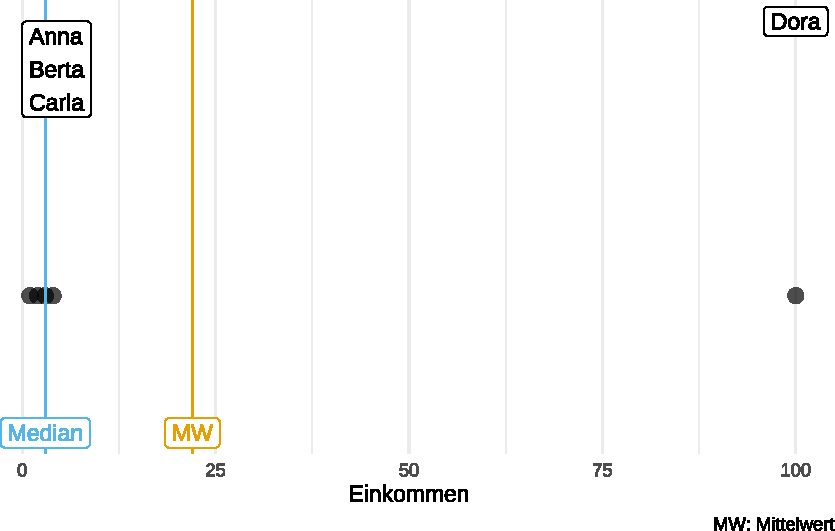
\includegraphics{050-zusammenfassen_files/figure-pdf/fig-md1-1.pdf}

}

\subcaption{\label{fig-md1-1}ID auf der X-Achse, Einkommen auf der
Y-Achse}

\end{minipage}%
\newline
\begin{minipage}{\linewidth}

\centering{

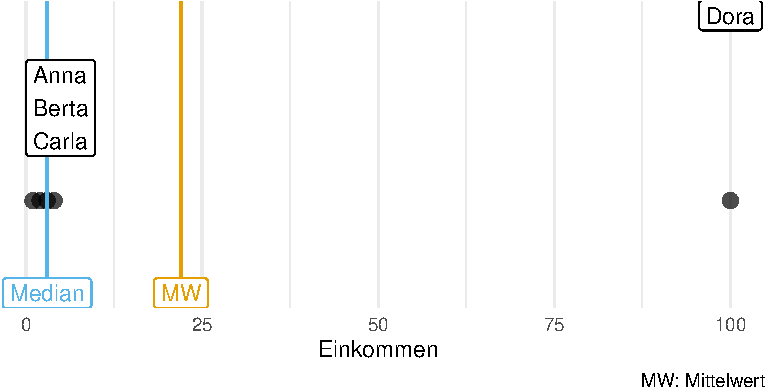
\includegraphics{050-zusammenfassen_files/figure-pdf/fig-md1-2.pdf}

}

\subcaption{\label{fig-md1-2}Einkommen auf der X-Achse, Häufigkeit auf
der Y-Achse}

\end{minipage}%

\caption{\label{fig-md1}Das Median-Einkommen einiger Studentinnen sowie
der Mittelwert (MW) ihres Einkommens}

\end{figure}%

Wir könnten jetzt behaupten, dass Carla das typische Einkommen (für
diese Datenreihe) aufweist, da es genauso viele Studentinnen gibt, die
mehr verdienen, wie solche, die weniger verdienen. \(\square\)

\end{example}

\begin{definition}[Median]\protect\hypertarget{def-median}{}\label{def-median}

Merkmalsausprägung, die bei (aufsteigend) sortierten Beobachtungen in
der Mitte liegt. \(\square\)

\end{definition}

\begin{exercise}[Alle mal
aufstehen]\protect\hypertarget{exr-aufstellen}{}\label{exr-aufstellen}

Auf Geheiß der Lehrkraft stehen jetzt alle Studis bitte auf und
sortieren sich der Größe nach im Raum, schön in einer Reihe aufgestellt.
Die Körpergröße der Person in der Mitte der Reihe, zu der also gleich
viele Personen zu links wie zu rechts stehen, das ist der Medien dieser
Datenreihe, vgl. Figure~\ref{fig-median-human}. \(\square\)

\end{exercise}

Der Median ist \emph{robust} (gegenüber) Extremwerten: Fügt man
Extremwerte zu einer Verteilung hinzu, ändert sich der Median zumeist
(deutlich) weniger als der Mittelwert.

Figure~\ref{fig-median-human} stellt den Median schematisch dar.

\begin{figure}

\begin{minipage}{0.20\linewidth}

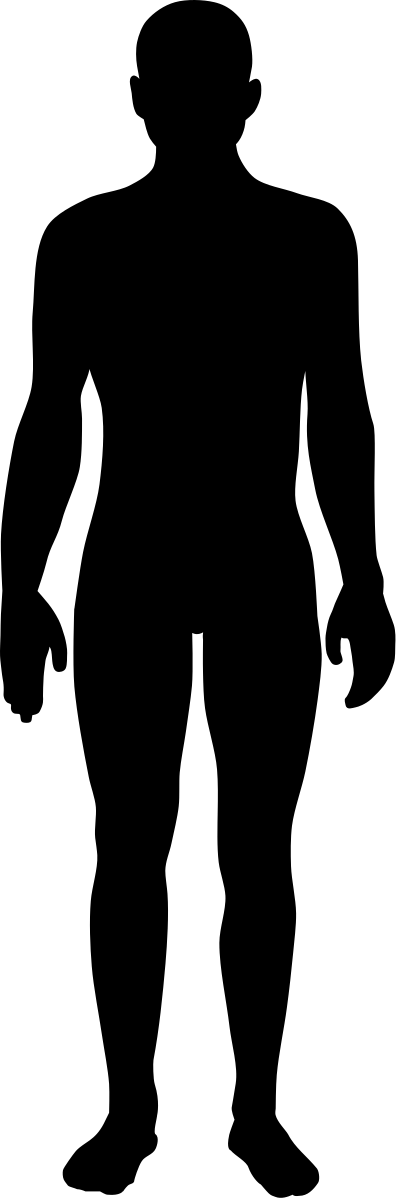
\includegraphics[width=0.1\textwidth,height=\textheight]{img/Human_Silhouette.svg.png}

\subcaption{\label{}1,60m}
\end{minipage}%
%
\begin{minipage}{0.20\linewidth}

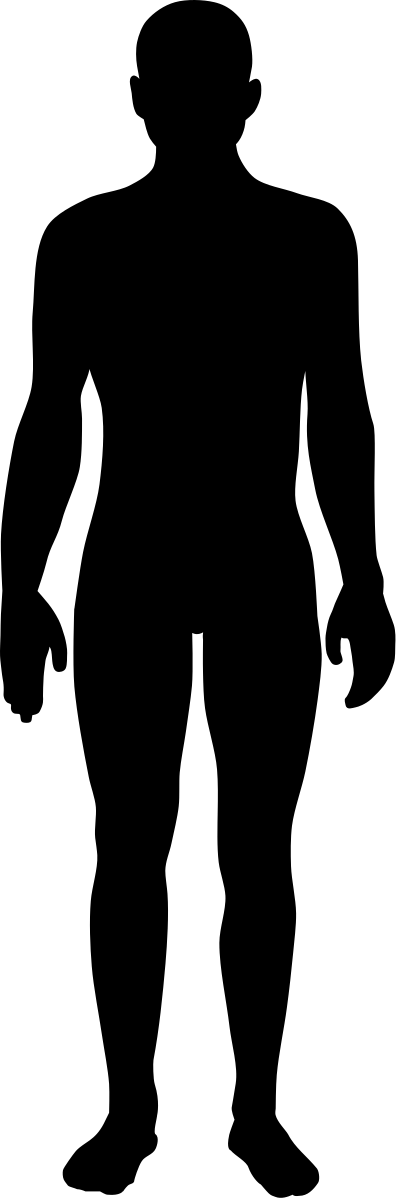
\includegraphics[width=0.13\textwidth,height=\textheight]{img/Human_Silhouette.svg.png}

\subcaption{\label{}1,72m}
\end{minipage}%
%
\begin{minipage}{0.20\linewidth}


\includegraphics[width=0.15\textwidth,height=\textheight]{img/human-red.png}

\subcaption{\label{}1,79m: Median!}
\end{minipage}%
%
\begin{minipage}{0.20\linewidth}

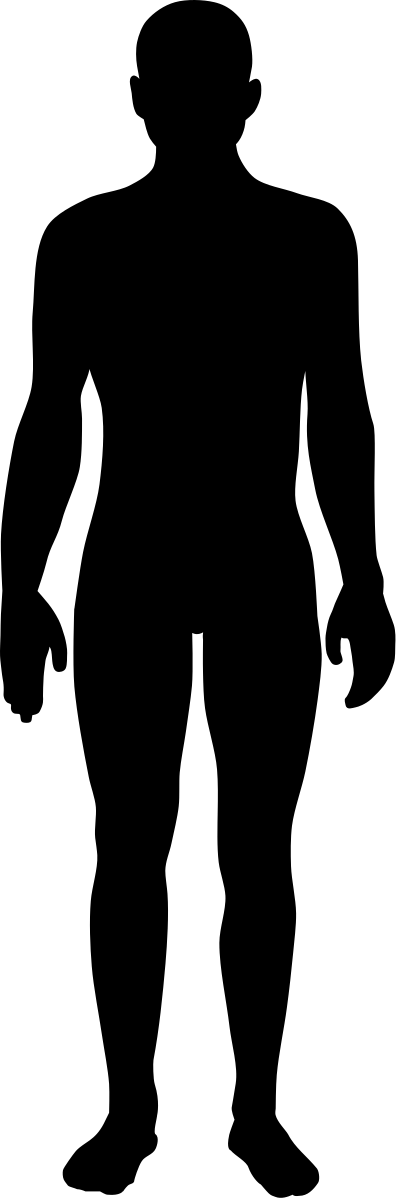
\includegraphics[width=0.16\textwidth,height=\textheight]{img/Human_Silhouette.svg.png}

\subcaption{\label{}1,94}
\end{minipage}%
%
\begin{minipage}{0.20\linewidth}

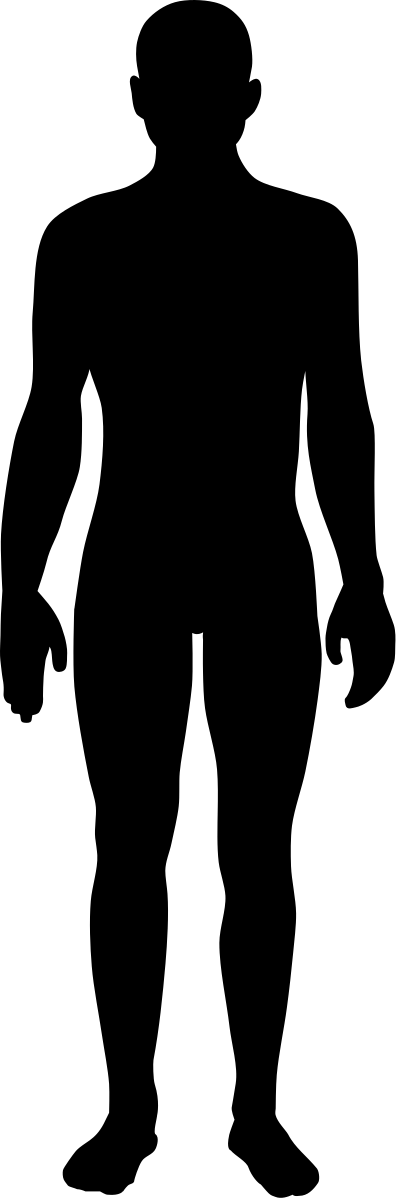
\includegraphics[width=0.2\textwidth,height=\textheight]{img/Human_Silhouette.svg.png}

\subcaption{\label{}2,12m}
\end{minipage}%

\caption{\label{fig-median-human}Der Median als der Wert des
``mittleren'' Objekts, wenn die Objekte aufsteigend sortiert sind. Es
gibt genauso viele Objekte mit kleinerem Wert als der Median wie Objekte
mit größerem Wert als der Median.}

\end{figure}%

Bei geradem \(n\) werden die beiden mittleren Werte betrachtet und das
arithmetische Mittel aus diesen beiden Werten gebildet.

\begin{example}[]\protect\hypertarget{exm-med2}{}\label{exm-med2}

Bei der Messreihe 1, 2, 3, 4, 5, 6, 8, 9 beträgt der Median
4.5.\(\square\)

\end{example}

\begin{exercise}[Emma wird
reich]\protect\hypertarget{exr-md2}{}\label{exr-md2}

Durch ein geniales Patent wird Emma steinreich. Ihr Einkommen erhöht
sich um das Hundertfache. Wie verändert sich der Median?\footnote{Er
  bleibt gleich, verändert sich also nicht: Der Median ist
  \emph{robust}, er verändert sich nicht oder kaum, wenn Extremwerte
  vorliegen.} \(\square\)

\end{exercise}

\begin{exercise}[Wer ist mehr ``mittel''? Median oder
Mittelwert?]\protect\hypertarget{exr-mw-md}{}\label{exr-mw-md}

~

\begin{quote}
🧑‍🎓 Das arithmetische Mittel sollte Mittelwert heißen, weil es die Mitte
von zwei Messwerten widerspiegelt, also z.B. von 1 und 10 ist die Mitte
5,5 - also genau beim Mittelwert!
\end{quote}

\begin{quote}
👩‍🎓 Moment! Der Median und nur der Median zeigt den mittleren Messwert!
Links und rechts sind gleich viele Messwerte, wenn man die Werte der
Größe nach sortiert. Also liegt der Median genau in der Mitte!
\end{quote}

Nehmen Sie Stellung zu dieser Diskussion!\(\square\)

\end{exercise}

\begin{example}[Ein ``mittlerer'' Preis für
Mariokart]\protect\hypertarget{exm-md3}{}\label{exm-md3}

Der Mittelwert (das arithmetische Mittel) und der Median für das
Start-Gebot (\texttt{start\_pr)} von Mariokart-Spielen sind nicht
gleich, der Mittelwert ist höher als der Median.

\begin{Shaded}
\begin{Highlighting}[]
\NormalTok{mariokart }\OtherTok{\textless{}{-}} \FunctionTok{read.csv}\NormalTok{(}\StringTok{"https://vincentarelbundock.github.io/Rdatasets/csv/openintro/mariokart.csv"}\NormalTok{)}

\NormalTok{mariokart }\SpecialCharTok{\%\textgreater{}\%} 
  \FunctionTok{summarise}\NormalTok{(}\AttributeTok{price\_mw =} \FunctionTok{mean}\NormalTok{(start\_pr),}
            \AttributeTok{price\_md =} \FunctionTok{median}\NormalTok{(start\_pr))}
\end{Highlighting}
\end{Shaded}

\begin{longtable}[]{@{}rr@{}}
\toprule\noalign{}
price\_mw & price\_md \\
\midrule\noalign{}
\endhead
\bottomrule\noalign{}
\endlastfoot
8.777203 & 1 \\
\end{longtable}

Wie man sieht, ist der Mittelwert größer als der Median, s.
Figure~\ref{fig-mario-md}

\begin{verbatim}
`stat_bin()` using `bins = 30`. Pick better value with
`binwidth`.
\end{verbatim}

\begin{figure}

\centering{

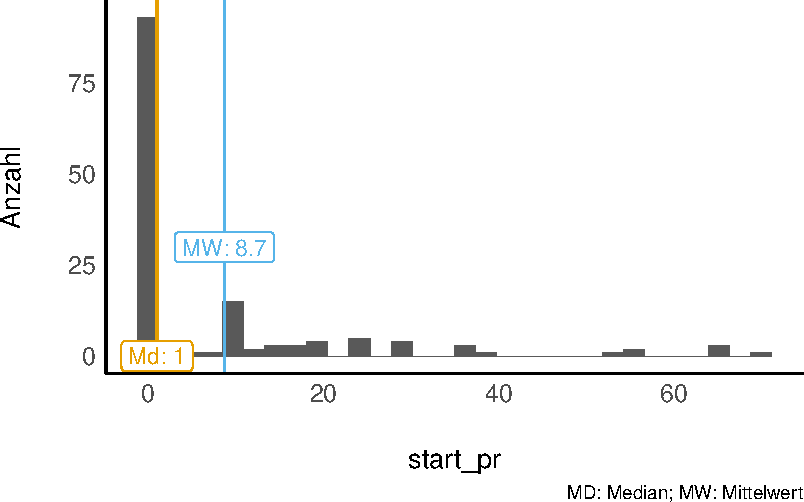
\includegraphics{050-zusammenfassen_files/figure-pdf/fig-mario-md-1.pdf}

}

\caption{\label{fig-mario-md}Das Start-Gebot bei Mariokart-Spielen ist
schief verteilt: Median und Mittelwert sind unterschiedlich}

\end{figure}%

\end{example}

\begin{tcolorbox}[enhanced jigsaw, breakable, toptitle=1mm, colback=white, leftrule=.75mm, colframe=quarto-callout-note-color-frame, colbacktitle=quarto-callout-note-color!10!white, title=\textcolor{quarto-callout-note-color}{\faInfo}\hspace{0.5em}{Note}, toprule=.15mm, opacityback=0, arc=.35mm, coltitle=black, rightrule=.15mm, titlerule=0mm, bottomtitle=1mm, bottomrule=.15mm, left=2mm, opacitybacktitle=0.6]

Klaffen Mittelwert und Median auseinander, so liegt eine schiefe
Verteilung vor. Ist der Mittelwert größer als der Median, so nennt man
die Verteilung rechtsschief. Bei schiefen Verteilungen ist der Median
dem Mittelwert als Modell für den ``typischen Wert'' vorzuziehen.

\end{tcolorbox}

\begin{exercise}[Mariokart ohne
Extremwerte]\protect\hypertarget{exr-mw-no-extrem}{}\label{exr-mw-no-extrem}

Im Datensatz \texttt{mariokart} gibt es einige wenige Spiele, die für
einen vergleichsweise hohen Preis verkauft wurden. Diese Extremwerte
verzerren den mittleren Verkaufspreis möglicherweise über die Gebühr.
\(\square\)

\end{exercise}

\subsubsection{Aufgabe}

Entfernen Sie diese Werte und berechnen Sie dann Mittelwert und Median
erneut. Vergleichen Sie die Ergebnisse.

\subsubsection{Lösung}

\begin{Shaded}
\begin{Highlighting}[]
\NormalTok{mariokart2 }\OtherTok{\textless{}{-}} 
\NormalTok{mariokart }\SpecialCharTok{\%\textgreater{}\%} 
  \FunctionTok{filter}\NormalTok{(total\_pr }\SpecialCharTok{\textless{}} \DecValTok{100}\NormalTok{)}

\CommentTok{\# ohne Extremwerte:}
\NormalTok{mariokart2 }\SpecialCharTok{|\textgreater{}} 
  \FunctionTok{summarise}\NormalTok{(}\AttributeTok{total\_pr\_mittelwert =} \FunctionTok{mean}\NormalTok{(total\_pr),}
            \AttributeTok{total\_pr\_median =} \FunctionTok{median}\NormalTok{(total\_pr))}
\end{Highlighting}
\end{Shaded}

\begin{longtable}[]{@{}rr@{}}
\toprule\noalign{}
total\_pr\_mittelwert & total\_pr\_median \\
\midrule\noalign{}
\endhead
\bottomrule\noalign{}
\endlastfoot
47.43191 & 46.03 \\
\end{longtable}

\begin{Shaded}
\begin{Highlighting}[]
\CommentTok{\# mit Extremwerten:}
\NormalTok{mariokart }\SpecialCharTok{|\textgreater{}} 
  \FunctionTok{summarise}\NormalTok{(}\AttributeTok{total\_pr\_mittelwert =} \FunctionTok{mean}\NormalTok{(total\_pr),}
            \AttributeTok{total\_pr\_median =} \FunctionTok{median}\NormalTok{(total\_pr))}
\end{Highlighting}
\end{Shaded}

\begin{longtable}[]{@{}rr@{}}
\toprule\noalign{}
total\_pr\_mittelwert & total\_pr\_median \\
\midrule\noalign{}
\endhead
\bottomrule\noalign{}
\endlastfoot
49.88049 & 46.5 \\
\end{longtable}

\begin{exercise}[]\protect\hypertarget{exr-mw-wealthmd}{}\label{exr-mw-wealthmd}

Was schätzen Sie, wie hoch das \emph{mediane} Vermögen des Haushalte in
Deutschland in etwa ist (Stand 2016)?\footnote{Quelle: WSI,
  \url{https://www.wsi.de/en/how-is-wealth-distributed-in-germany-14401.htm},
  Abruf 2023-04-19. Die Antwort lautet: ca. 60 Tsd Euro laut der
  angegebenen Quelle.})

\begin{enumerate}
\def\labelenumi{\alph{enumi})}
\tightlist
\item
  50.000 Euro
\item
  100.000 Euro
\item
  150.000 Euro
\item
  200.000 Euro
\item
  250.000 Euro\(\square\)
\end{enumerate}

\end{exercise}

\begin{exercise}[]\protect\hypertarget{exr-mw-wealthmd}{}\label{exr-mw-wealthmd}

Was schätzen Sie, wie groß der \emph{Unterschied} zwischen medianem und
mittlerem (arithm. Mittel) des Jahreseinkommen deutscher Haushalte
ungefähr ist?\footnote{Quelle:
  \href{https://de.wikipedia.org/wiki/Einkommensverteilung_in_Deutschland}{Wikipedia},
  Abruf 2023-04-19, der Unterschied beträgt knapp 3000 Euro laut der
  Quelle.})

\begin{enumerate}
\def\labelenumi{\alph{enumi})}
\tightlist
\item
  1.000 Euro
\item
  2.000 Euro
\item
  3.000 Euro
\item
  4.000 Euro
\item
  5.000 Euro\(\square\)
\end{enumerate}

\end{exercise}

\subsection{Quantile}\label{quantile}

Der Median teilt eine Verteilung in eine untere und ein obere Hälfte. Er
markiert sozusagen eine ``50-Prozent-Marke'' (der aufsteigend sortierten
Beobachtungen). Betrachten wir einmal nur alle Spiele, die für weniger
als 100 Euro verkauft wurden (\texttt{total\_pr}, finales
Verkaufsgebot), s. Figure~\ref{fig-quantile-mario}. 50\% aller Spiele
wurden für weniger als ca. 46 Euro verkauft; 50\% aller Spiele für mehr
als 46 Euro. Der Median beträgt als 46 Euro.

Jetzt könnten wir nur die günstigere Hälfte betrachten und wieder nach
dem Median fragen (d.h. \texttt{total\_pr\ \textless{}\ 46}). Dieser
``Median der günstigeren Hälfte'' grenzt damit das insgesamt günstigste
Viertel vom Rest der Verkaufsgebote ab. In unserem Datensatz liegt
dieser Wert bei ca. 41 Euro. Entsprechend kann man nach dem Wert fragen,
der das oberste Viertel vom Rest der Verkaufsgebote abtrennt. Dieser
Wert liegt bei ca. 54 Euro.

\begin{definition}[Quartile]\protect\hypertarget{def-quartile}{}\label{def-quartile}

Sortiert man die Daten aufsteigend, so nennt man den Wert, der das
Viertel mit den kleisten Wert vom Rest der Daten trennt das \emph{erste
Quartil} (Q1, 25\%). Den Median nennt man das \emph{zweite Quartil} (Q2,
50\%). Entsprechend heißt der Wert, der die drei Viertel kleinsten Werte
vom oberen Viertel abtrennt, das \emph{dritte Quartil} (Q3,
75\%).\(\square\)

\end{definition}

\begin{example}[Quartile des
Verkaufsgebot]\protect\hypertarget{exm-mario-qs}{}\label{exm-mario-qs}

Figure~\ref{fig-quantile-mario} zeigt die Quartile für das
Verkaufsgebot.\(\square\)

\end{example}

Jetzt könnte man sagen, hey, warum nur in 25\%-Stücke die Verteilung
aufteilen? Warum nicht in 10\%-Schritten?

\begin{definition}[Dezile]\protect\hypertarget{def-dezile}{}\label{def-dezile}

Die neun Quantile \(p= 0.1, 0.2, \ldots, 1\), die die Verteilung in 10
gleiche Teile unterteilen, nennt man Dezile. \(\square\)

\end{definition}

Oder vielleicht in 1\%-Schritten oder in sonstigen Schnitten? Wo die
Quartile in 25\%-Schritten aufteilen, teilt in \emph{Quantil} in
\(p\)-Prozent-Schritten auf.

\begin{definition}[Quantile]\protect\hypertarget{def-quantile}{}\label{def-quantile}

Ein p-Quantil ist der Wert, der von \(p\) Prozent der Werte nicht
überschritten wird.\(\square\)

\end{definition}

\begin{tcolorbox}[enhanced jigsaw, breakable, toptitle=1mm, colback=white, leftrule=.75mm, colframe=quarto-callout-note-color-frame, colbacktitle=quarto-callout-note-color!10!white, title=\textcolor{quarto-callout-note-color}{\faInfo}\hspace{0.5em}{Note}, toprule=.15mm, opacityback=0, arc=.35mm, coltitle=black, rightrule=.15mm, titlerule=0mm, bottomtitle=1mm, bottomrule=.15mm, left=2mm, opacitybacktitle=0.6]

Ein Quantil ist ein Oberbegriff für Quartile, Dezile, etc. \(\square\)

\end{tcolorbox}

Figure~\ref{fig-quantile-mario} zeigt das 1. (Q1), das 2. (Median) und
das 3. Quartil für den Datensatz \texttt{mariokart2}.

\begin{figure}

\centering{

\subsubsection{Histogramm}

\begin{verbatim}
`stat_bin()` using `bins = 30`. Pick better value with
`binwidth`.
\end{verbatim}

\centering{

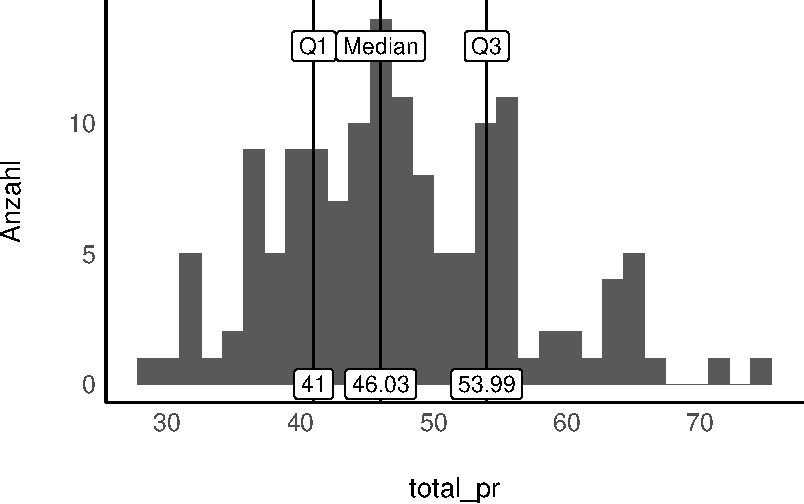
\includegraphics{050-zusammenfassen_files/figure-pdf/fig-mario-qs1-1.pdf}

}

\subcaption{\label{fig-mario-qs1}Q1, Q2 und Q3 für das Schlussgebot (nur
Spiele für weniger als 100 Euro)}

\subsubsection{Dichtediagramm}

\centering{

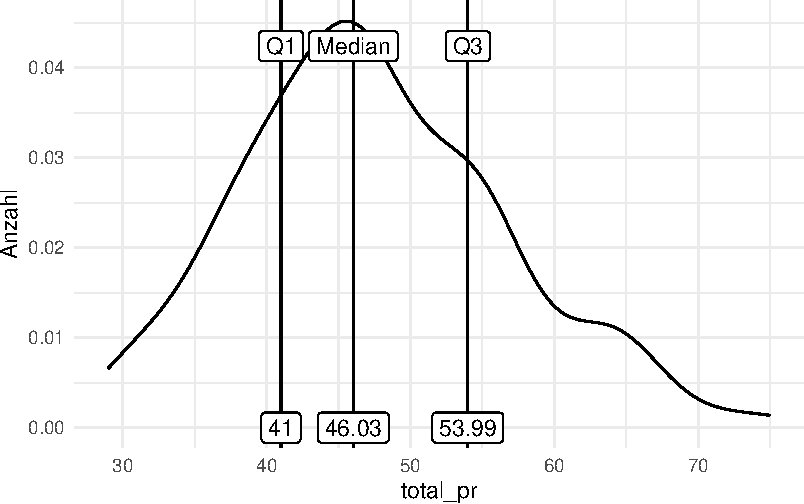
\includegraphics{050-zusammenfassen_files/figure-pdf/fig-mario-qs2-1.pdf}

}

\subcaption{\label{fig-mario-qs2}Q1, Q2 und Q3 für das Schlussgebot (nur
Spiele für weniger als 100 Euro)}

}

\caption{\label{fig-quantile-mario}Verschiedene Arten von Quantilen.}

\end{figure}%

\emph{Quantile} kann man in R mit dem Befehl \texttt{quantile()}
berechnen:

\begin{Shaded}
\begin{Highlighting}[]
\NormalTok{mario\_quantile }\OtherTok{\textless{}{-}} 
\NormalTok{mariokart }\SpecialCharTok{\%\textgreater{}\%} 
  \FunctionTok{filter}\NormalTok{(total\_pr }\SpecialCharTok{\textless{}} \DecValTok{100}\NormalTok{) }\SpecialCharTok{\%\textgreater{}\%} 
  \FunctionTok{summarise}\NormalTok{(}\AttributeTok{q25 =} \FunctionTok{quantile}\NormalTok{(total\_pr, .}\DecValTok{25}\NormalTok{),}
            \AttributeTok{q50 =} \FunctionTok{quantile}\NormalTok{(total\_pr, .}\DecValTok{50}\NormalTok{),}
            \AttributeTok{q75 =} \FunctionTok{quantile}\NormalTok{(total\_pr, .}\DecValTok{75}\NormalTok{))}
\end{Highlighting}
\end{Shaded}

Figure~\ref{fig-quantile-mosaic} visualisiert verschiedene Quantile. Man
beachte, dass alle Regionen gleichgroße Flächen (d.h.
Wahrscheinlichkeitsmassen) aufweisen.

\begin{figure}

\centering{

\subsubsection{Quartile}

\begin{verbatim}
\end{verbatim}

\begin{verbatim}
If X ~ N(0, 1), then 
\end{verbatim}

\begin{verbatim}
    P(X <= -0.6744898) = 0.25   P(X <=  0.0000000) = 0.50   P(X <=  0.6744898) = 0.75
\end{verbatim}

\begin{verbatim}
    P(X >  -0.6744898) = 0.75   P(X >   0.0000000) = 0.50   P(X >   0.6744898) = 0.25
\end{verbatim}

\begin{verbatim}
\end{verbatim}

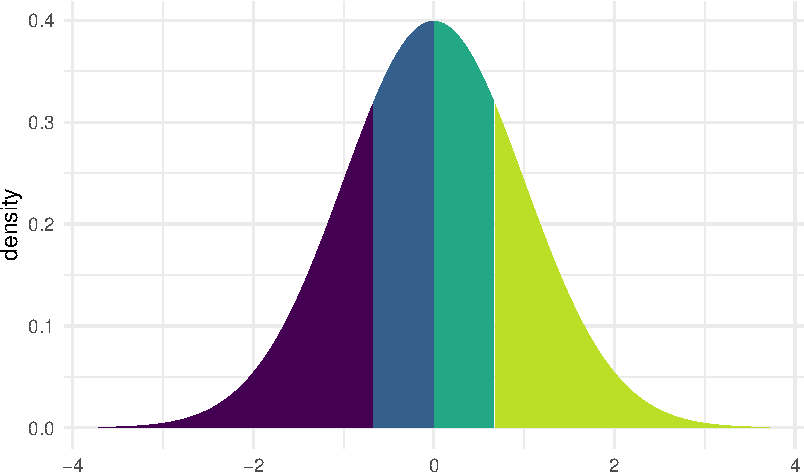
\includegraphics{050-zusammenfassen_files/figure-pdf/unnamed-chunk-17-1.pdf}

\subsubsection{Dezile}

\begin{verbatim}
\end{verbatim}

\begin{verbatim}
If X ~ N(0, 1), then 
\end{verbatim}

\begin{verbatim}
    P(X <=       -Inf) = 0.0    P(X <= -1.2815516) = 0.1    P(X <= -0.8416212) = 0.2    P(X <= -0.5244005) = 0.3    P(X <= -0.2533471) = 0.4    P(X <=  0.0000000) = 0.5    P(X <=  0.2533471) = 0.6    P(X <=  0.5244005) = 0.7    P(X <=  0.8416212) = 0.8    P(X <=  1.2815516) = 0.9    P(X <=        Inf) = 1.0
\end{verbatim}

\begin{verbatim}
    P(X >        -Inf) = 1.0    P(X >  -1.2815516) = 0.9    P(X >  -0.8416212) = 0.8    P(X >  -0.5244005) = 0.7    P(X >  -0.2533471) = 0.6    P(X >   0.0000000) = 0.5    P(X >   0.2533471) = 0.4    P(X >   0.5244005) = 0.3    P(X >   0.8416212) = 0.2    P(X >   1.2815516) = 0.1    P(X >         Inf) = 0.0
\end{verbatim}

\begin{verbatim}
\end{verbatim}

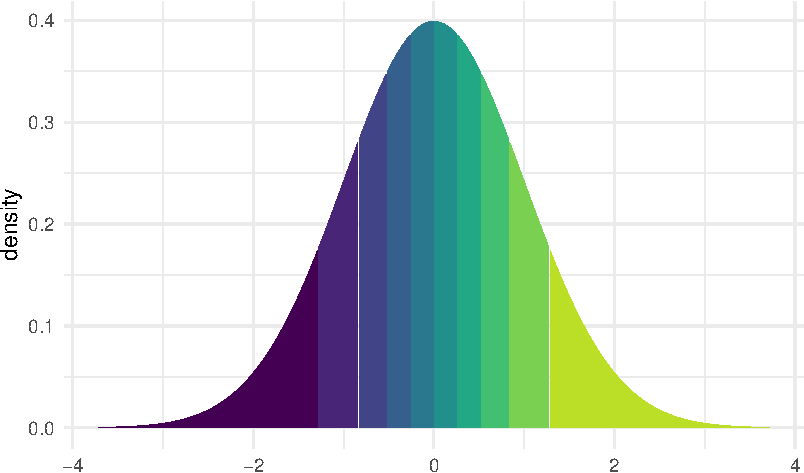
\includegraphics{050-zusammenfassen_files/figure-pdf/unnamed-chunk-18-1.pdf}

\subsubsection{Perzentile}

\begin{verbatim}
\end{verbatim}

\begin{verbatim}
If X ~ N(0, 1), then 
\end{verbatim}

\begin{verbatim}
    P(X <=        -Inf) = 0.00  P(X <= -2.32634787) = 0.01  P(X <= -2.05374891) = 0.02  P(X <= -1.88079361) = 0.03  P(X <= -1.75068607) = 0.04  P(X <= -1.64485363) = 0.05  P(X <= -1.55477359) = 0.06  P(X <= -1.47579103) = 0.07  P(X <= -1.40507156) = 0.08  P(X <= -1.34075503) = 0.09  P(X <= -1.28155157) = 0.10  P(X <= -1.22652812) = 0.11  P(X <= -1.17498679) = 0.12  P(X <= -1.12639113) = 0.13  P(X <= -1.08031934) = 0.14  P(X <= -1.03643339) = 0.15  P(X <= -0.99445788) = 0.16  P(X <= -0.95416525) = 0.17  P(X <= -0.91536509) = 0.18  P(X <= -0.87789630) = 0.19  P(X <= -0.84162123) = 0.20  P(X <= -0.80642125) = 0.21  P(X <= -0.77219321) = 0.22  P(X <= -0.73884685) = 0.23  P(X <= -0.70630256) = 0.24  P(X <= -0.67448975) = 0.25  P(X <= -0.64334541) = 0.26  P(X <= -0.61281299) = 0.27  P(X <= -0.58284151) = 0.28  P(X <= -0.55338472) = 0.29  P(X <= -0.52440051) = 0.30  P(X <= -0.49585035) = 0.31  P(X <= -0.46769880) = 0.32  P(X <= -0.43991317) = 0.33  P(X <= -0.41246313) = 0.34  P(X <= -0.38532047) = 0.35  P(X <= -0.35845879) = 0.36  P(X <= -0.33185335) = 0.37  P(X <= -0.30548079) = 0.38  P(X <= -0.27931903) = 0.39  P(X <= -0.25334710) = 0.40  P(X <= -0.22754498) = 0.41  P(X <= -0.20189348) = 0.42  P(X <= -0.17637416) = 0.43  P(X <= -0.15096922) = 0.44  P(X <= -0.12566135) = 0.45  P(X <= -0.10043372) = 0.46  P(X <= -0.07526986) = 0.47  P(X <= -0.05015358) = 0.48  P(X <= -0.02506891) = 0.49  P(X <=  0.00000000) = 0.50  P(X <=  0.02506891) = 0.51  P(X <=  0.05015358) = 0.52  P(X <=  0.07526986) = 0.53  P(X <=  0.10043372) = 0.54  P(X <=  0.12566135) = 0.55  P(X <=  0.15096922) = 0.56  P(X <=  0.17637416) = 0.57  P(X <=  0.20189348) = 0.58  P(X <=  0.22754498) = 0.59  P(X <=  0.25334710) = 0.60  P(X <=  0.27931903) = 0.61  P(X <=  0.30548079) = 0.62  P(X <=  0.33185335) = 0.63  P(X <=  0.35845879) = 0.64  P(X <=  0.38532047) = 0.65  P(X <=  0.41246313) = 0.66  P(X <=  0.43991317) = 0.67  P(X <=  0.46769880) = 0.68  P(X <=  0.49585035) = 0.69  P(X <=  0.52440051) = 0.70  P(X <=  0.55338472) = 0.71  P(X <=  0.58284151) = 0.72  P(X <=  0.61281299) = 0.73  P(X <=  0.64334541) = 0.74  P(X <=  0.67448975) = 0.75  P(X <=  0.70630256) = 0.76  P(X <=  0.73884685) = 0.77  P(X <=  0.77219321) = 0.78  P(X <=  0.80642125) = 0.79  P(X <=  0.84162123) = 0.80  P(X <=  0.87789630) = 0.81  P(X <=  0.91536509) = 0.82  P(X <=  0.95416525) = 0.83  P(X <=  0.99445788) = 0.84  P(X <=  1.03643339) = 0.85  P(X <=  1.08031934) = 0.86  P(X <=  1.12639113) = 0.87  P(X <=  1.17498679) = 0.88  P(X <=  1.22652812) = 0.89  P(X <=  1.28155157) = 0.90  P(X <=  1.34075503) = 0.91  P(X <=  1.40507156) = 0.92  P(X <=  1.47579103) = 0.93  P(X <=  1.55477359) = 0.94  P(X <=  1.64485363) = 0.95  P(X <=  1.75068607) = 0.96  P(X <=  1.88079361) = 0.97  P(X <=  2.05374891) = 0.98  P(X <=  2.32634787) = 0.99  P(X <=         Inf) = 1.00
\end{verbatim}

\begin{verbatim}
    P(X >         -Inf) = 1.00  P(X >  -2.32634787) = 0.99  P(X >  -2.05374891) = 0.98  P(X >  -1.88079361) = 0.97  P(X >  -1.75068607) = 0.96  P(X >  -1.64485363) = 0.95  P(X >  -1.55477359) = 0.94  P(X >  -1.47579103) = 0.93  P(X >  -1.40507156) = 0.92  P(X >  -1.34075503) = 0.91  P(X >  -1.28155157) = 0.90  P(X >  -1.22652812) = 0.89  P(X >  -1.17498679) = 0.88  P(X >  -1.12639113) = 0.87  P(X >  -1.08031934) = 0.86  P(X >  -1.03643339) = 0.85  P(X >  -0.99445788) = 0.84  P(X >  -0.95416525) = 0.83  P(X >  -0.91536509) = 0.82  P(X >  -0.87789630) = 0.81  P(X >  -0.84162123) = 0.80  P(X >  -0.80642125) = 0.79  P(X >  -0.77219321) = 0.78  P(X >  -0.73884685) = 0.77  P(X >  -0.70630256) = 0.76  P(X >  -0.67448975) = 0.75  P(X >  -0.64334541) = 0.74  P(X >  -0.61281299) = 0.73  P(X >  -0.58284151) = 0.72  P(X >  -0.55338472) = 0.71  P(X >  -0.52440051) = 0.70  P(X >  -0.49585035) = 0.69  P(X >  -0.46769880) = 0.68  P(X >  -0.43991317) = 0.67  P(X >  -0.41246313) = 0.66  P(X >  -0.38532047) = 0.65  P(X >  -0.35845879) = 0.64  P(X >  -0.33185335) = 0.63  P(X >  -0.30548079) = 0.62  P(X >  -0.27931903) = 0.61  P(X >  -0.25334710) = 0.60  P(X >  -0.22754498) = 0.59  P(X >  -0.20189348) = 0.58  P(X >  -0.17637416) = 0.57  P(X >  -0.15096922) = 0.56  P(X >  -0.12566135) = 0.55  P(X >  -0.10043372) = 0.54  P(X >  -0.07526986) = 0.53  P(X >  -0.05015358) = 0.52  P(X >  -0.02506891) = 0.51  P(X >   0.00000000) = 0.50  P(X >   0.02506891) = 0.49  P(X >   0.05015358) = 0.48  P(X >   0.07526986) = 0.47  P(X >   0.10043372) = 0.46  P(X >   0.12566135) = 0.45  P(X >   0.15096922) = 0.44  P(X >   0.17637416) = 0.43  P(X >   0.20189348) = 0.42  P(X >   0.22754498) = 0.41  P(X >   0.25334710) = 0.40  P(X >   0.27931903) = 0.39  P(X >   0.30548079) = 0.38  P(X >   0.33185335) = 0.37  P(X >   0.35845879) = 0.36  P(X >   0.38532047) = 0.35  P(X >   0.41246313) = 0.34  P(X >   0.43991317) = 0.33  P(X >   0.46769880) = 0.32  P(X >   0.49585035) = 0.31  P(X >   0.52440051) = 0.30  P(X >   0.55338472) = 0.29  P(X >   0.58284151) = 0.28  P(X >   0.61281299) = 0.27  P(X >   0.64334541) = 0.26  P(X >   0.67448975) = 0.25  P(X >   0.70630256) = 0.24  P(X >   0.73884685) = 0.23  P(X >   0.77219321) = 0.22  P(X >   0.80642125) = 0.21  P(X >   0.84162123) = 0.20  P(X >   0.87789630) = 0.19  P(X >   0.91536509) = 0.18  P(X >   0.95416525) = 0.17  P(X >   0.99445788) = 0.16  P(X >   1.03643339) = 0.15  P(X >   1.08031934) = 0.14  P(X >   1.12639113) = 0.13  P(X >   1.17498679) = 0.12  P(X >   1.22652812) = 0.11  P(X >   1.28155157) = 0.10  P(X >   1.34075503) = 0.09  P(X >   1.40507156) = 0.08  P(X >   1.47579103) = 0.07  P(X >   1.55477359) = 0.06  P(X >   1.64485363) = 0.05  P(X >   1.75068607) = 0.04  P(X >   1.88079361) = 0.03  P(X >   2.05374891) = 0.02  P(X >   2.32634787) = 0.01  P(X >          Inf) = 0.00
\end{verbatim}

\begin{verbatim}
\end{verbatim}

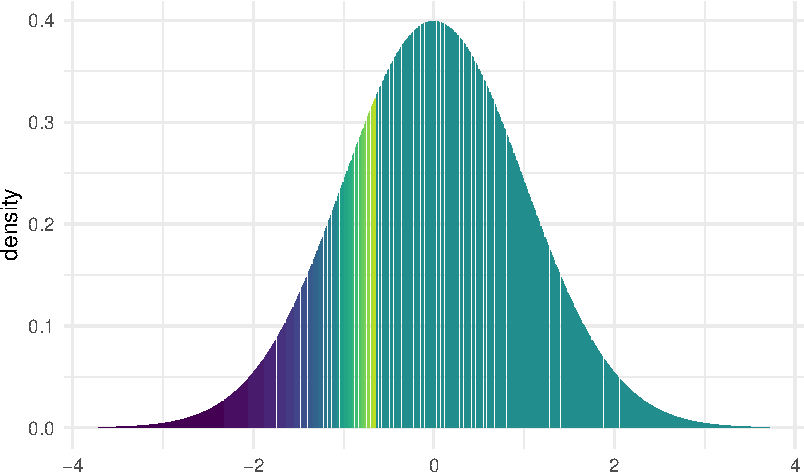
\includegraphics{050-zusammenfassen_files/figure-pdf/unnamed-chunk-19-1.pdf}

}

\caption{\label{fig-quantile-mosaic}Verschiedene Quantile visualisiert.
In jedem Diagramm sind die Regionen gleich groß, beinhalten also
(ungefähr) die gleiche Anzahl von Beobachtungen.}

\end{figure}%

\subsection{Lagemaße}\label{sec-lage}

\begin{quote}
{\emoji{student}} Was ist der Oberbegriff für Median, Mittelwert und so
weiter?
\end{quote}

\begin{quote}
{\emoji{teacher}} Gute Frage! Wie würden Sie ihn nennen?
\end{quote}

\begin{definition}[Lagemaß]\protect\hypertarget{def-lage}{}\label{def-lage}

Ein \emph{Lagemaß} (synonym: Maß der zentralen Tendenz) für eine
Verteilung gibt einen Vorschlag, welchen Wert der Verteilung wir als
typisch, normal, erwartbar, repräsentativ oder ``mittel'' ansehen
sollten.\(\square\)

\end{definition}

\begin{example}[]\protect\hypertarget{exm-lagemaße}{}\label{exm-lagemaße}

Gebräuchliche Lagemaße sind:

\begin{itemize}
\tightlist
\item
  Mittelwert (arithmetisches Mittel)
\item
  Median
\item
  Quartile
\item
  Quantile
\item
  Minimum (kleinster Wert)
\item
  Maximum (größter Wert)
\item
  Modus (häufigster Wert) \(\square\)
\end{itemize}

\end{example}

Berechnen wir Lagemaße für den Mariokart-Datensatz, s.
Listing~\ref{lst-mario-lage}.\footnote{Es ist übrigens egal, wie sie die
  Variablen benennen, die Sie berechnen: \texttt{mw} oder
  \texttt{mittelwert} oder \texttt{mean} oder
  \texttt{mein\_krasser\_variablenname} -- alles okay!}

\begin{codelisting}

\caption{\label{lst-mario-lage}Syntax zur Berechnung von Lagemaßen}

\centering{

\begin{Shaded}
\begin{Highlighting}[]
\NormalTok{mariokart\_lagemaße\_total\_pr }\OtherTok{\textless{}{-}}
\NormalTok{  mariokart }\SpecialCharTok{\%\textgreater{}\%} 
  \FunctionTok{summarise}\NormalTok{(}\AttributeTok{mw =} \FunctionTok{mean}\NormalTok{(total\_pr),}
            \AttributeTok{md =} \FunctionTok{median}\NormalTok{(total\_pr),}
            \AttributeTok{q1 =} \FunctionTok{quantile}\NormalTok{(total\_pr, .}\DecValTok{25}\NormalTok{),}
            \AttributeTok{q2 =} \FunctionTok{quantile}\NormalTok{(total\_pr, .}\DecValTok{5}\NormalTok{),}
            \AttributeTok{q3 =} \FunctionTok{quantile}\NormalTok{(total\_pr, .}\DecValTok{75}\NormalTok{),}
            \AttributeTok{min =} \FunctionTok{min}\NormalTok{(total\_pr),}
            \AttributeTok{max =} \FunctionTok{max}\NormalTok{(total\_pr))}
\NormalTok{mariokart\_lagemaße\_total\_pr}
\end{Highlighting}
\end{Shaded}

\begin{longtable*}[]{@{}rrrrrrr@{}}
\toprule\noalign{}
mw & md & q1 & q2 & q3 & min & max \\
\midrule\noalign{}
\endhead
\bottomrule\noalign{}
\endlastfoot
49.88049 & 46.5 & 41.175 & 46.5 & 53.99 & 28.98 & 326.51 \\
\end{longtable*}

}

\end{codelisting}%

\subsubsection{Gruppierte Lagemaße}\label{gruppierte-lagemauxdfe}

Häufig möchte man Statistiken wie Lagemaße für mehrere Teilgruppen --
z.B. Mittlere Körpergröße von Frauen vs.~Mittlere Körpergröße von Männer
-- berechnen und dann vergleichen. Die zugrundeliegende stehende
\emph{Forschungsfrage} könnte lauten:

\begin{quote}
Unterscheidet sich die mittlere Körpergröße von Frauen und Männern?
\end{quote}

Oder vielleicht:

\begin{quote}
Hat das Geschlecht einen Einfluss auf die Körpergröße?
\end{quote}

Anders ausgedrückt:

\begin{quote}
Körpergröße \(\color{ycol}{\text{y}}\) ist eine Funktion des Geschlechts
\(\color{xcol}{G}\).
\end{quote}

Die \emph{Modellformel} könnte also lauten:

\[\color{ycol}{y} \; \color{black}{ \sim } \; \color{xcol}{G}\]

Gruppierte Lagemaße lassen sich in R z.B. so berechnen, s.
Listing~\ref{lst-mario-lage-gruppiert}, also ähnlich wie in
Listing~\ref{lst-mario-lage}.

\begin{codelisting}

\caption{\label{lst-mario-lage-gruppiert}Gruppierte Lagemaße}

\centering{

\begin{Shaded}
\begin{Highlighting}[]
\NormalTok{mariokart\_lagemaße\_gruppiert }\OtherTok{\textless{}{-}}
\NormalTok{  mariokart }\SpecialCharTok{\%\textgreater{}\%} 
  \FunctionTok{group\_by}\NormalTok{(wheels) }\SpecialCharTok{\%\textgreater{}\%}  \CommentTok{\# neue Zeile, der Rest ist gleich!}
  \FunctionTok{summarise}\NormalTok{(}\AttributeTok{mw =} \FunctionTok{mean}\NormalTok{(total\_pr))}

\NormalTok{mariokart\_lagemaße\_gruppiert}
\end{Highlighting}
\end{Shaded}

\begin{longtable*}[]{@{}rr@{}}
\toprule\noalign{}
wheels & mw \\
\midrule\noalign{}
\endhead
\bottomrule\noalign{}
\endlastfoot
0 & 41.05973 \\
1 & 44.16885 \\
2 & 61.02745 \\
3 & 69.75000 \\
4 & 65.02000 \\
\end{longtable*}

}

\end{codelisting}%

Figure~\ref{fig-mw3} zeigt ein Beispiel für ungruppierte (links) bzw.
gruppierte (rechts) Mittelwerte; vgl. Figure~\ref{fig-mw2}. Wie man in
dem Diagramm sieht, kann das \emph{Residuum kleiner} werden bei einer
Gruppierung (im Vergleich zu einem ungruppierten, ``globalen''
Mittelwert): Innerhalb der Gruppe ohne Lenkräder und innerhalb der
Gruppe mit 2 Lenkrädern sind die Abweichungen zu ihrem
Gruppen-Mittelwert relativ gering -- im Vergleich zu den Abweichungen
der Preise zum ungruppierten Mittelwert.

\begin{figure}

\begin{minipage}{0.50\linewidth}

\centering{

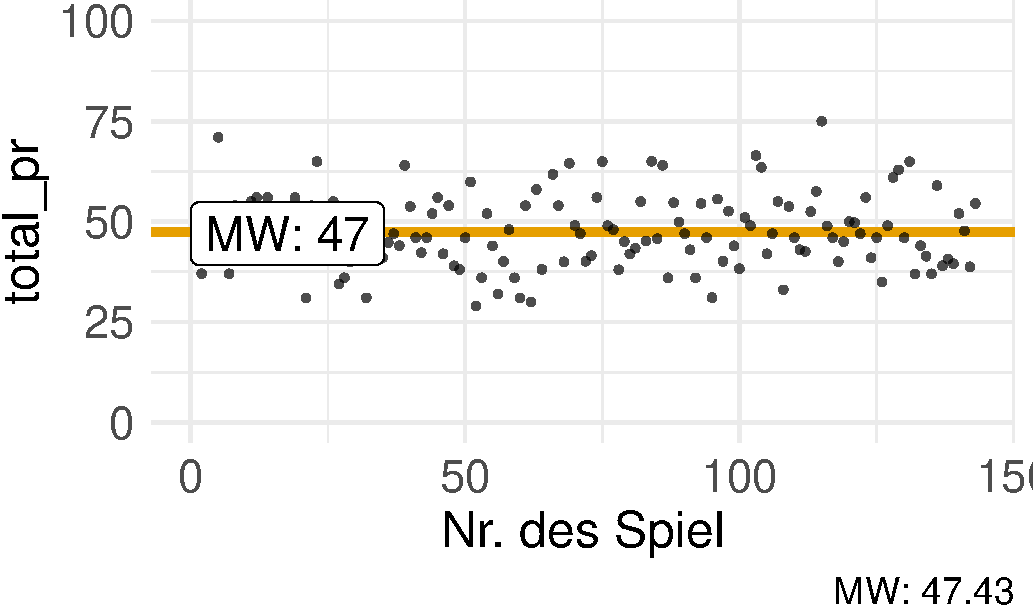
\includegraphics{050-zusammenfassen_files/figure-pdf/fig-mw3-1.pdf}

}

\subcaption{\label{fig-mw3-1}Mittelwert für Verkaufspreis (ungruppiert)}

\end{minipage}%
%
\begin{minipage}{0.50\linewidth}

\centering{

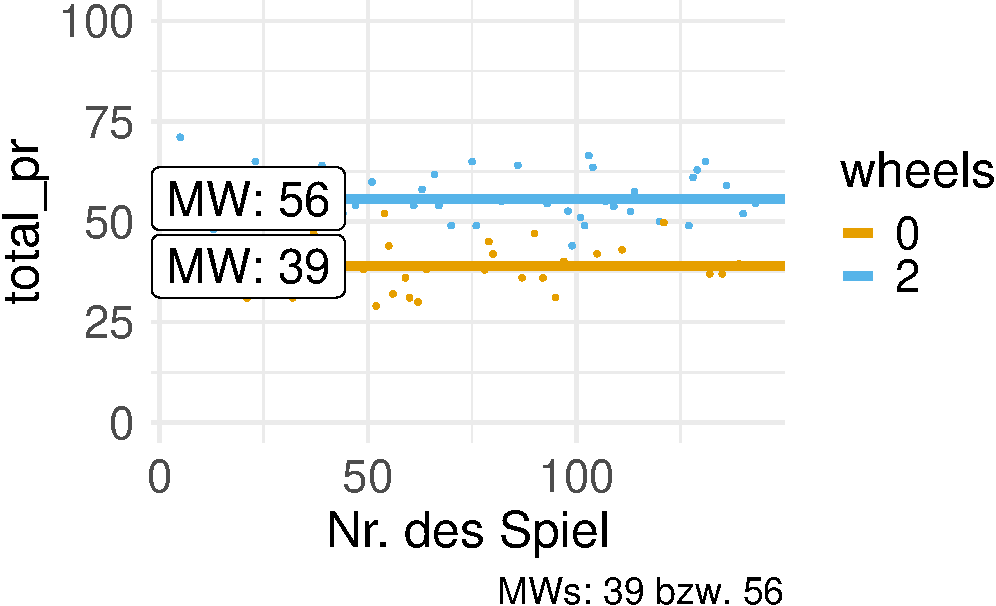
\includegraphics{050-zusammenfassen_files/figure-pdf/fig-mw3-2.pdf}

}

\subcaption{\label{fig-mw3-2}Mittelwert für Verkaufspreis gruppiert nach
Anzahl der Lenkräder}

\end{minipage}%

\caption{\label{fig-mw3}Der mittlere Preis von Mariokart-Spielen als
horizontale Gerade eingezeichnet}

\end{figure}%

\begin{definition}[Punktmodell]\protect\hypertarget{def-punktmodell}{}\label{def-punktmodell}

Ein Modell, welches für alle Beobachtungen ein und denselben Wert
annimmt (vorhersagt), heißt ein \emph{Punktmodell}. Anders gesagt fasst
ein Punktmodell eine Wertereihe (häufig ist das eine Tabellenspalte) zu
einer einzelnen Zahl zusammen, einem ``Punkt'' in diesem Sinne, s.
Equation~\ref{eq-desk}.\(\square\)

\end{definition}

\begin{equation}\phantomsection\label{eq-desk}{\begin{array}{|c|} \hline \\ \hline \\\\\\ \hline \end{array} \qquad \rightarrow \qquad \begin{array}{|c|} \hline \\ \hline  \hline \end{array}}\end{equation}

Mittelwert, Median und Quartile sind Beispiele für Punktmodelle: Sie
fassen eine Verteilung zu einem einzelnen Wert zusammen und geben uns
ein ``Bild'' der Daten, machen Sie uns verständlich - sie sind uns ein
Modell.

\subsection{Wie man mit Statistik
lügt}\label{wie-man-mit-statistik-luxfcgt}

Mit Statistik kann man vortrefflich lügen, heißt es. Woran liegt das?
Der Grund ist, dass die Statistik Freiheitsgrade lässt: Es gibt nicht
nur einen richtigen Weg, um eine statistische Analyse durchzuführen.
Viele Wege führen nach Rom (aber nicht alle). Um Manipulationsversuche
abzuwehren oder einfache Fehler und Unschärfen ohne böse Abwehr
aufzudecken, gibt es ein probates Gegenmittel: \emph{Transparenz}.

\phantomsection\label{callout-important}
Stellen Sie hohe Anforderung an die Transparenz einer statistischen
Analyse. Nur durch Nachprüfbarkeit können Sie sich von der
Stichhaltigkeit der Ergebnisse und deren Interpretation überzeugen.

Hier ist eine (nicht abschließende!) Checkliste, was Sie nachprüfen
sollten, um die Belastbarkeit einer Analyse sicherzustellen
{[}@simmons\_false-positive\_2011, @wicherts\_degrees\_2016-1{]}:

\begin{longtable*}{rl}
\toprule
Nr & Check \\ 
\midrule\addlinespace[2.5pt]
1 & Wurde die Art und die Zeitdauer der Datenerhebung vorab festgelegt und berichtet? \\ 
2 & Wurden ausreichend Daten gesammelt (z.B. mind. 20 Beobachtungen pro Gruppe)? \\ 
3 & Wurden alle untersuchten Variablen berichtet? \\ 
4 & Wurden alle durchgeführten Interventionen berichtet? \\ 
5 & Wurden Daten aus der Analyse entfernt? Wenn ja, gibt es eine (stichhaltige) Begründung? \\ 
\bottomrule
\end{longtable*}

\subsection{Vertiefung}\label{vertiefung}

\begin{example}[Survival-Tipp]\protect\hypertarget{exm-survival1}{}\label{exm-survival1}

Eine Studentin aus dem dem Bachelorstudiengang ``Angewandte Medien- und
Wirtschaftspsychologie'' mit Schwerpunkt \emph{Data Science} berichtet
ihre ``Survival-Tipps'' für Statistik.

\begin{enumerate}
\def\labelenumi{\arabic{enumi}.}
\tightlist
\item
  Wenn man mal nicht weiterkommt, hilft es auch mal ein paar Tage
  Abstand von R und Statistik zu nehmen.
\item
  Es hilft, sich während des Semesters neue Begriffe und ihre Erklärung
  zusammenschreiben.
\item
  Gut ist auch, sich mit KommilitonInnen auszutauschen oder in höheren
  Semestern nach Tipps fragen.\(\square\)
\end{enumerate}

\end{example}

\begin{quote}
{\emoji{student}} Irgendwie kann ich mir R-Code so schlecht merken.
\end{quote}

\begin{quote}
{\emoji{teacher}} Frag doch mal ChatGPT, oder einen anderen Chatbot, da
bekommt man auch R-Code ausgegegeben.
\end{quote}

\begin{exercise}[Übungsfragen vom
Chat-Bot]\protect\hypertarget{exr-chatgpt}{}\label{exr-chatgpt}

Fragen Sie einen Chat-Bot wie ChatGPT nach Übungsaufgaben.

Sie können sich an folgenden Prompt orientieren. Empfehlenswert ist mit
verschiedenen Prompts zu experimentieren.

\begin{quote}
🧑‍🎓 Ich bin ein Student in einem Bachelor-Studiengang für Psychologie.
Gerade bereite ich mich auf die Klausur im Fach ``Grundlagen der
Statistik'' vor. Bitte schreibe mir Aufgaben, die mir helfen, mich auf
die Prüfung vorzubereiten. Die Fragen sollten folgende Themen
beinhalten: Maße der zentralen Tendenz, Grundlagen von R, Skalenniveau
(z.B. Nominalskala vs.~Intervallskala), Verteilungsformen,
Normalverteilungen, z-Werte. Bitte schreibe die Aufgabe im Stil von
Richtig-Falsch-Aufgaben. Schreibe ca. 10 Aufgaben.
\end{quote}

\(\square\)

\end{exercise}

\subsection{Aufgaben}\label{aufgaben}

Ein Teil der folgenden Aufgaben kann Stoff beinhalten, den Sie noch
nicht kennen, aber später kennenlernen. Ignorieren Sie daher
Aufgaben(teile) mit (noch) unbekannte Stoff.

Die Webseite \href{https://datenwerk.netlify.app}{datenwerk.netlify.app}
stellt eine Reihe von einschlägigen Übungsaufgaben bereit. Sie können
die Suchfunktion der Webseite nutzen, um die Aufgaben mit den folgenden
Namen zu suchen:

\begin{enumerate}
\def\labelenumi{\arabic{enumi}.}
\tightlist
\item
  \href{https://datenwerk.netlify.app/posts/kennwert-robust/kennwert-robust}{Kennwert-robust}
\item
  \href{https://datenwerk.netlify.app/posts/mw-berechnen/mw-berechnen.html}{mw-berechnen}
\item
  \href{https://datenwerk.netlify.app/posts/mariokart-max2/mariokart-max2.html}{mariokart-max2}
\item
  \href{https://datenwerk.netlify.app/posts/nasa01/nasa01.html}{nasa01}
\item
  \href{https://datenwerk.netlify.app/posts/mariokart-mean1/mariokart-mean1.html}{mariokart-mean1}
\item
  \href{https://datenwerk.netlify.app/posts/wrangle10/wrangle10.html}{wrangle10}
\item
  \href{https://datenwerk.netlify.app/posts/summarise01/summarise01.html}{summarise01}
\item
  \href{https://datenwerk.netlify.app/posts/mariokart-max1/mariokart-max1.html}{mariokart-max1}
\item
  \href{https://datenwerk.netlify.app/posts/schiefe1/schiefe1}{Schiefe1}
\item
  \href{https://datenwerk.netlify.app/posts/mariokart-mean2/mariokart-mean2.html}{mariokart-mean2}
\item
  \href{https://datenwerk.netlify.app/posts/summarise03/summarise03.html}{summarise03}
\item
  \href{https://datenwerk.netlify.app/posts/mariokart-mean4/mariokart-mean4.html}{mariokart-mean4}
\item
  \href{https://datenwerk.netlify.app/posts/mariokart-mean3/mariokart-mean3.html}{mariokart-mean3}
\item
  \href{https://datenwerk.netlify.app/posts/summarise02/summarise02.html}{summarise02}
\end{enumerate}

\begin{tcolorbox}[enhanced jigsaw, breakable, toptitle=1mm, colback=white, leftrule=.75mm, colframe=quarto-callout-tip-color-frame, colbacktitle=quarto-callout-tip-color!10!white, title=\textcolor{quarto-callout-tip-color}{\faLightbulb}\hspace{0.5em}{Tip}, toprule=.15mm, opacityback=0, arc=.35mm, coltitle=black, rightrule=.15mm, titlerule=0mm, bottomtitle=1mm, bottomrule=.15mm, left=2mm, opacitybacktitle=0.6]

Schauen Sie sich auch mal auf
\href{https://datenwerk.netlify.app}{datenwerk.netlify.app} die Aufgaben
zu z.B. dem Tag \href{https://datenwerk.netlify.app/\#category=eda}{EDA}
an. \(\square\)

\end{tcolorbox}

\begin{exercise}[]\protect\hypertarget{exr-datensaetze}{}\label{exr-datensaetze}

Mittlerweile verfügen Sie die wesentlichen Werkzeuge des Datenjudo.
\href{https://data-se.netlify.app/2022/02/23/data-sets-for-for-teaching/}{Hier}
finden Sie einen Überblick an Datensätze, die Sie nach Herzenslust
analysieren können.\footnote{\url{https://data-se.netlify.app/2022/02/23/data-sets-for-for-teaching/}}
\(\square\)

\end{exercise}

\subsection{Literaturhinweise}\label{literaturhinweise}

Es gibt viele Lehrbücher zu den Grundlagen der Statistik; die Inhalte
dieses Kapitels gehören zu den Grundlagen der Statistik. Vielleicht ist
es am einfachsten, wenn Sie einfach in Ihrer Bibliothek des Vertrauens
nach einem typischen Lehrbuch schauen. Beispiel für Lehrbücher sind
@mittag\_statistik\_2020 oder @oestreich\_keine\_2014; ein Klassiker ist
@bortz\_statistik\_2010. Ein Fokus auf R legt @sauer\_moderne\_2019-1.
Wer vor Englisch nicht zurückschreckt, ist mit
@cetinkaya-rundel\_introduction\_2021-2 oder
@poldrack\_statistical\_2022-1 gut beraten. Beide Bücher sind online
verfügbar. Tipp: Mit dem Browser einfach auf Deutsch übersetzen.

\subsection{Literatur}\label{literatur}




\end{document}
